\documentclass[12pt]{article}
\usepackage[margin=1in]{geometry}
\usepackage{amsmath}
\usepackage{amsfonts}
\usepackage{amssymb}
\usepackage{amsthm}
\usepackage{graphicx}
\usepackage{tikz}
\usetikzlibrary{arrows}
\usepackage{esvect}
\usepackage{pgfplots}

\title{Math 218-1 Workbook}
\author{Aaron Greicius, Gabriela Laboska}
\date{Last update 09/14/2026}

\newenvironment{solution}{\begin{proof}[Solution]}{\end{proof}}
%\newenvironment{read}{\renewcommand{\qedsymbol} \begin{proof}[Required reading]}{\end{proof}}
\newenvironment{reading}{%
	\renewcommand{\qedsymbol}{}%
	\begin{proof}[Reading]%
	}{%
	\end{proof}%
}
\begin{document}
	
	\maketitle
	\vspace{2cm}
	\begin{itemize}
		\item This workbook was made to be a companion to the already existing Math 218-1 textbook. It contains exercises to help you better understand the material and prepare for any upcoming exams/quizzes.
		\item This workbook will be updated regularly, so please make sure to have the latest version at all times.
		\item If you notice any typos or inconsistencies, please email Gabriela Laboska 
		
		(gabriela.laboska@northwestern.edu).
	\end{itemize}
	
	\newpage
	
	\tableofcontents
	\newpage
	
	\section{What is a function?}
	
	\begin{enumerate}
		\item Write the following sets using interval notation and sketch them on the real number line. Your answer should be an interval or a union of intervals.
		\begin{enumerate}
			\item $\{x\in\mathbb{R}| -1\leq x<5\}$
			\begin{solution}
				$[-1,5)$.
				\begin{center}
				
				
				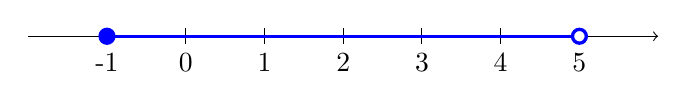
\begin{tikzpicture}
					% Number line
					\draw[->] (-2,0) -- (6,0);
					
					% Tick marks
					\foreach \x in {-1,0,1,2,3,4,5}
					\draw (\x,0.1) -- (\x,-0.1);
					
					% Labels
					\foreach \x in {-1,0,1,2,3,4,5}
					\node[below] at (\x,-0.1) {\x};
					
					% Interval
					\draw[very thick, blue] (-1,0) -- (5,0);
					
					% Closed endpoint at -1
					\draw[very thick, blue, fill=blue] (-1,0) circle (2.5pt);
					
					% Open endpoint at 5
					\draw[very thick, blue, fill=white] (5,0) circle (2.5pt);
				\end{tikzpicture}
			\end{center}
			\end{solution}
			\item $\{x\in\mathbb{R}| x>2 \text{ or } x<-2\}$
			\begin{solution}
				$(-\infty,-2)\cup (2,\infty)$.
				\begin{center}
		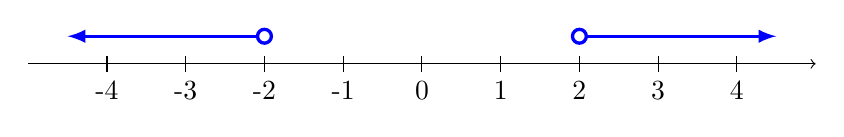
\begin{tikzpicture}
			% Number line
			\draw[->] (-5,0) -- (5,0);
			
			% Tick marks
			\foreach \x in {-4,-3,-2,-1,0,1,2,3,4}
			\draw (\x,0.1) -- (\x,-0.1);
			
			% Labels
			\foreach \x in {-4,-3,-2,-1,0,1,2,3,4}
			\node[below] at (\x,-0.1) {\x};
			
			% Blue interval
			\draw[very thick, blue, -latex] (-2,0.35) -- (-4.5,0.35);
			\draw[very thick, blue, -latex] (2,0.35) -- (4.5,0.35);
			
			% Hollow endpoints
			\draw[very thick, blue, fill=white] (-2,0.35) circle (2.5pt);
			\draw[very thick, blue, fill=white] (2,0.35) circle (2.5pt);
		\end{tikzpicture}
		\end{center}
			\end{solution}
			\item $\{x\in\mathbb{R}| x \text{ is a nonnegative number whose absolute value is less than } 3\}$
			\begin{solution}
				$[0,3)$.
				\begin{center}
				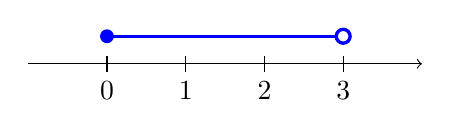
\begin{tikzpicture}
					% Number line
					\draw[->] (-1,0) -- (4,0);
					
					% Tick marks
					\foreach \x in {0,1,2,3}
					\draw (\x,0.1) -- (\x,-0.1);
					
					% Labels
					\foreach \x in {0,1,2,3}
					\node[below] at (\x,-0.1) {\x};
					
					% Blue interval
					\draw[very thick, blue] (0,0.35) -- (3,0.35);
					
					% Closed endpoint at 0
					\fill[blue] (0,0.35) circle (2.5pt);
					
					% Open endpoint at 3
					\draw[very thick, blue, fill=white] (3,0.35) circle (2.5pt);
				\end{tikzpicture}
				\end{center}
			\end{solution}
		\end{enumerate}
		\item Consider the graphs given below. Determine which of them are graphs of functions.

		\begin{enumerate}
			\item 
			
		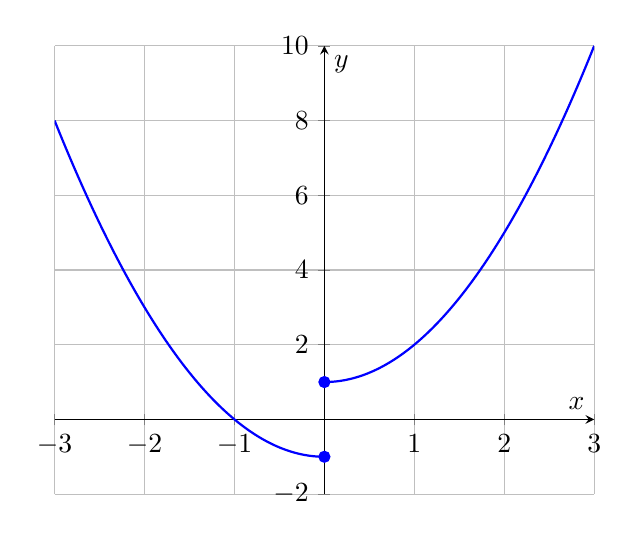
\begin{tikzpicture}
			\begin{axis}[
				axis lines = middle,
				xlabel = {$x$},
				ylabel = {$y$},
				xmin = -3, xmax = 3,
				ymin = -2, ymax = 10,
				grid = both
				]
				
				% f(x) = x^2 - 1 for x <= 0
				\addplot[
				domain=-3:0,
				samples=100,
				blue,
				thick
				] {x^2 - 1};
				
				% f(x) = x^2 + 1 for x >= 0
				\addplot[
				domain=0:3,
				samples=100,
				blue,
				thick
				] {x^2 + 1};
				
				\addplot[
				only marks,
				mark=*,
				mark size=2pt,
				blue
				] coordinates {(0,-1)};
				
				\addplot[
				only marks,
				mark=*,
				mark size=2pt,
				blue
				] coordinates {(0,1)};
				
				
			\end{axis}
			
		
		\end{tikzpicture}
		\begin{solution}
			Not a function. The $y$-axis is a vertical line that intersects the graph at 2 points. Therefore, the graph fails the vertical line test.
		\end{solution}
		
		\item 
		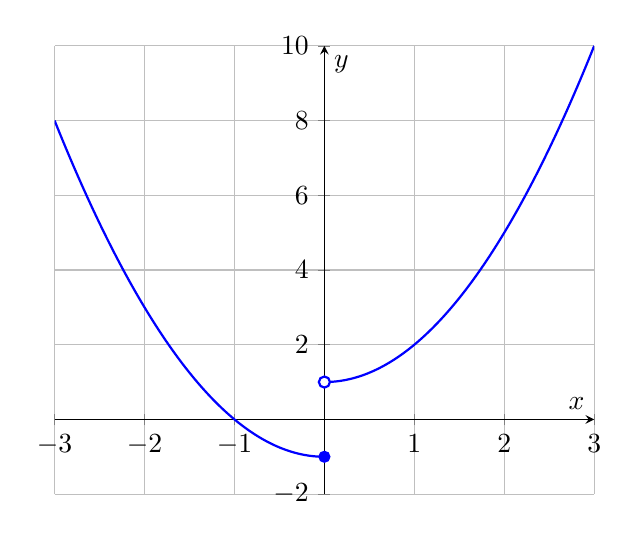
\begin{tikzpicture}
			\begin{axis}[
				axis lines = middle,
				xlabel = {$x$},
				ylabel = {$y$},
				xmin = -3, xmax = 3,
				ymin = -2, ymax = 10,
				grid = both
				]
				
				% f(x) = x^2 - 1 for x <= 0
				\addplot[
				domain=-3:0,
				samples=100,
				blue,
				thick
				] {x^2 - 1};
				
				% f(x) = x^2 + 1 for x >= 0
				\addplot[
				domain=0:3,
				samples=100,
				blue,
				thick
				] {x^2 + 1};
				
				\addplot[
				only marks,
				mark=*,
				mark size=2pt,
				blue
				] coordinates {(0,-1)};
				
				\addplot[
				only marks,
				mark=*,
				mark size=2pt,
				fill=white,
				draw=blue,
				thick
				] coordinates {(0,1)};
				
			\end{axis}
			
			
		\end{tikzpicture}
		\begin{solution}
			This is a graph of a function. Every vertical line intersects the graph at at most one point.
		\end{solution}
		\item
	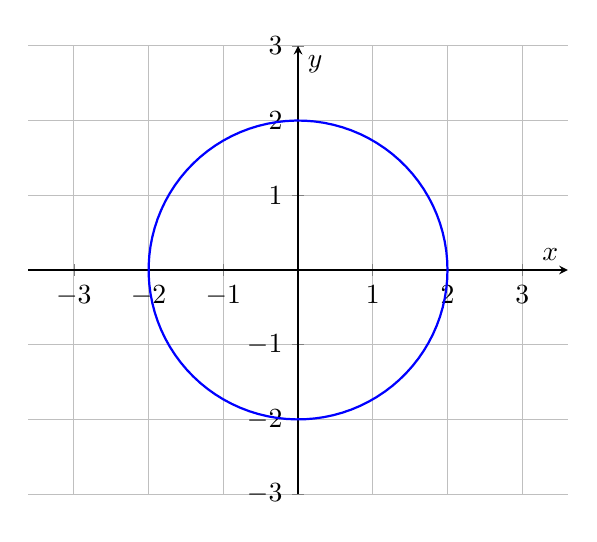
\begin{tikzpicture}
		\begin{axis}[
			axis lines = middle,
			xlabel = {$x$},
			ylabel = {$y$},
			xmin = -3, xmax = 3,
			ymin = -3, ymax = 3,
			xtick={-3,-2,-1,0,1,2,3},
			ytick={-3,-2,-1,0,1,2,3},
			grid = both,
			axis equal
			]
			
			% Circle x^2 + y^2 = 4
			\addplot[
			domain=0:360,
			samples=100,
			blue,
			thick
			] ({2*cos(x)}, {2*sin(x)});
			
		\end{axis}
	\end{tikzpicture}
	\begin{solution}
		Not a function. The $y$-axis is a vertical line that intersects the graph at two points. Therefore, the graph fails the vertical line test.
	\end{solution}
	\item 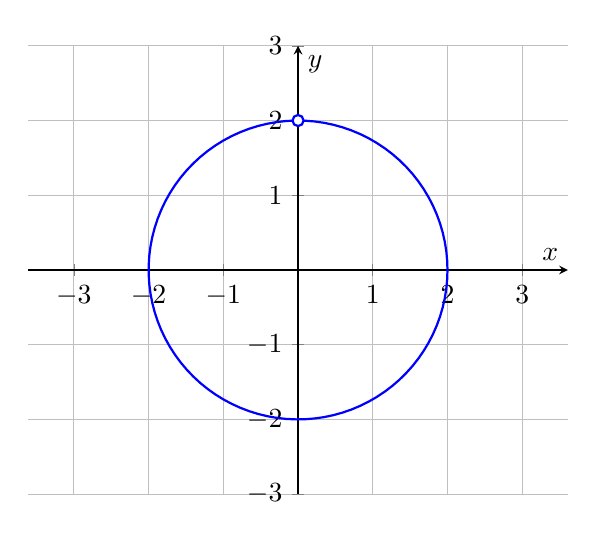
\begin{tikzpicture}
		\begin{axis}[
			axis lines = middle,
			xlabel = {$x$},
			ylabel = {$y$},
			xmin = -3, xmax = 3,
			ymin = -3, ymax = 3,
			xtick={-3,-2,-1,0,1,2,3},
			ytick={-3,-2,-1,0,1,2,3},
			grid = both,
			axis equal
			]
			
			% Circle x^2 + y^2 = 4
			\addplot[
			domain=0:360,
			samples=100,
			blue,
			thick
			] ({2*cos(x)}, {2*sin(x)});
			
			% Hole at (2,0)
			\addplot[
			only marks,
			mark=*,
			mark size=2pt,
			fill=white,
			draw=blue,
			thick
			] coordinates {(0,2)};
			
		\end{axis}
	\end{tikzpicture}
	\begin{solution}
		While the $y$-axis intersects the graph at only one point, the vertical line $x=1$ intersects it at two points. Therefore, this is not the graph of a function.
	\end{solution}
	\end{enumerate}
	
		\item The graphs of some functions are given below. Assume that the functions are defined only on the given grid.
		\begin{itemize}
			\item Find the domain and range of the functions based on the graphs. Your answer should be an interval or a union of intervals.
			\item For each function, find the values of $f(0), f(1), f(-1)$, or state that a value does not exist.
			\item For each function, find all the values of $x$ such that $f(x)=0$ (if any).
		\end{itemize}
		\begin{enumerate}
			\item 
			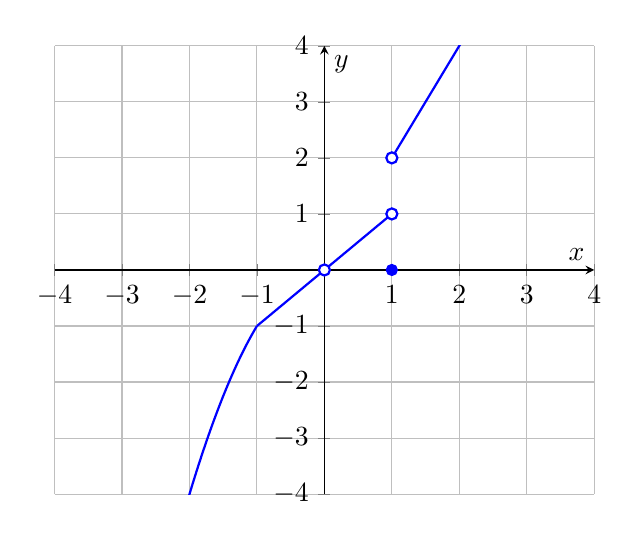
\begin{tikzpicture}
				\begin{axis}[
					axis lines = middle,
					xlabel = {$x$},
					ylabel = {$y$},
					xmin = -4, xmax = 4,
					ymin = -4, ymax = 4,
					xtick={-4,-3,-2,-1,0,1,2,3,4},
					ytick={-4,-3,-2,-1,0,1,2,3,4},
					grid = both
					]
					
					% Concave down quadratic on (-infty,-1)
					\addplot[
					domain=-3:-1,
					samples=100,
					blue,
					thick
					] {-x^2};
					
					% Linear function on (-1,1)
					\addplot[
					domain=-1:1,
					samples=100,
					blue,
					thick
					] {x};
					
					% Concave up quadratic y = x^2 + 1 on (1,infty)
					\addplot[
					domain=1:3,
					samples=100,
					blue,
					thick
					] {2*x};
					
					% Hole at (1,2)
					\addplot[
					only marks,
					mark=*,
					mark size=2pt,
					fill=white,
					draw=blue,
					thick
					] coordinates {(1,2)};
					
					% Hole at (1,1)
					\addplot[
					only marks,
					mark=*,
					mark size=2pt,
					fill=white,
					draw=blue,
					thick
					] coordinates {(1,1)};
					
						% Hole at (0,0)
					\addplot[
					only marks,
					mark=*,
					mark size=2pt,
					fill=white,
					draw=blue,
					thick
					] coordinates {(0,0)};
					
					% Point at (1,0)
					\addplot[
					only marks,
					mark=*,
					mark size=2pt,
					blue
					] coordinates {(1,0)};
					
				\end{axis}
			\end{tikzpicture}
			
			\begin{solution}
				\begin{itemize}
					\item The domain is $[-2,0)\cup (0,2)$, the range is $[-4,1)\cup(2,4]$.
					\item $f(0)$ does not exist, $f(1)=0$ and $f(-1)=-1$.
					\item $x=1$.
				\end{itemize}
			\end{solution}
			
			
			\item 
			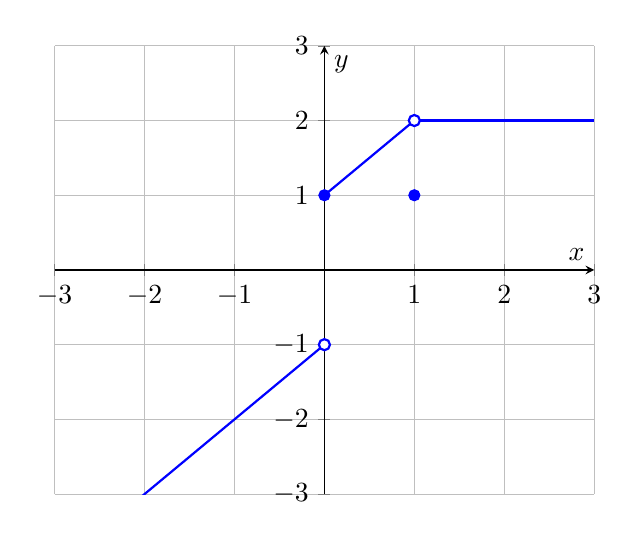
\begin{tikzpicture}
				\begin{axis}[
					axis lines = middle,
					xlabel = {$x$},
					ylabel = {$y$},
					xmin = -3, xmax = 3,
					ymin = -3, ymax = 3,
					xtick={-3,-2,-1,0,1,2,3},
					ytick={-3,-2,-1,0,1,2,3},
					grid = both
					]
					
					% y = x - 1 for x < 0
					\addplot[
					domain=-3:0,
					samples=100,
					blue,
					thick
					] {x - 1};
					
					% y = x + 1 for 0 < x < 1
					\addplot[
					domain=0:1,
					samples=100,
					blue,
					thick
					] {x + 1};
					
					% y = 2 for x > 1
					\addplot[
					domain=1:3,
					samples=100,
					blue,
					thick
					] {2};
					
					% Hole at (0,-1)
					\addplot[
					only marks,
					mark=*,
					mark size=2pt,
					fill=white,
					draw=blue,
					thick
					] coordinates {(0,-1)};
					
					% Point at (0,1)
					\addplot[
					only marks,
					mark=*,
					mark size=2pt,
					blue
					] coordinates {(0,1)};
					
					% Hole at (1,2)
					\addplot[
					only marks,
					mark=*,
					mark size=2pt,
					fill=white,
					draw=blue,
					thick
					] coordinates {(1,2)};
					
					% Point at (1,1)
					\addplot[
					only marks,
					mark=*,
					mark size=2pt,
					blue
					] coordinates {(1,1)};
					
				\end{axis}
			\end{tikzpicture}
			\begin{solution}
				\begin{itemize}
					\item The domain is $[-2,3]$ and the range is $[-3,-1)\cup[1,2]$.
					\item $f(0)=1,f(1)=1,f(-1)=-2$.
					\item There are no $x$ such that $f(x)=0$.
				\end{itemize}
			\end{solution}			
		\end{enumerate}
		
		\item Determine whether the following statements are true or false. Justify your reasoning.
		\begin{enumerate}
			\item It is not possible for two intervals to intersect at exactly one point.
			\begin{solution}
				False. For example, the intervals $(-1,1]$ and $[1,2]$ intersect at exactly one point.
			\end{solution}
			\item A function assigns exactly one output to each input.
			\begin{solution}
				True. This is part of the definition of a function.
			\end{solution}
			\item The following points are points on the graph of a function $(0,2),(1,1),(1,2),(2,1)$.
			\begin{solution}
				False. The input 1 has two outputs 1 and 2.
			\end{solution}
			\item The following points are points on the graph of a function $(0,2),(1,2),(2,1),(-1,1)$.
			\begin{solution}
				True. Every input has exactly one output (even though two different inputs have the same output).
			\end{solution}
			\item
				If the range of a function consists of only one point, the domain also consists of only one point.
			\begin{solution}
				False. It is possible for different inputs of a function to have the same output. An example is the function $f$ with domain $\{1,2\}$ and range $\{3\}$, defined by $f(1)=3,f(2)=3$ (or any other constant function).
			\end{solution}
		\end{enumerate}
	\end{enumerate}
	
	\newpage
	\section{Linear and Quadratic Functions}
		\begin{enumerate}
		\item Determine which of the following functions are linear. For those that are:
		\begin{itemize} 
			\item Find the $x$ and $y$-intercepts (if any)
			\item Determine whether they are increasing or decreasing
			\item Find the $x$ for which the function is positive/negative.
			\item Find the minimum/maximum (if any).
			\item Sketch the graph of the function.
		\end{itemize}
		\begin{enumerate}
			\item $f(x)=-\dfrac{1}{2}x+2$
		
			\begin{solution}
				
				The function is linear. 
				
				To find the $x$-intercept, we need to solve the equation $-\dfrac{1}{2}x+2=0$. Solving the equation, we get $x=4$, so the $x$-intercept is $(4,0)$.
				
				To find the $y$-intercept, set $x=0$. We get $y=2$, so the $y$-intercept is $(0,2)$. 
				
				Since the slope $m=-\dfrac{1}{2}<0$, the function is decreasing on $\mathbb{R}$, and hence, has no minimum/maximum.
				
				To find the $x$ for which the function is positive/negative, we need to solve the inequalities $f(x)>0$ and $f(x)<0$. Note that it is enough to solve one of them.
				$$f(x)>0$$
				$$-\dfrac{1}{2}x+2>0$$
				$$-\dfrac{1}{2}x>-2$$
				$$x<4.$$
				Therefore, the function is positive on $(-\infty,4)$ and negative on $(4,\infty)$.
				
				
				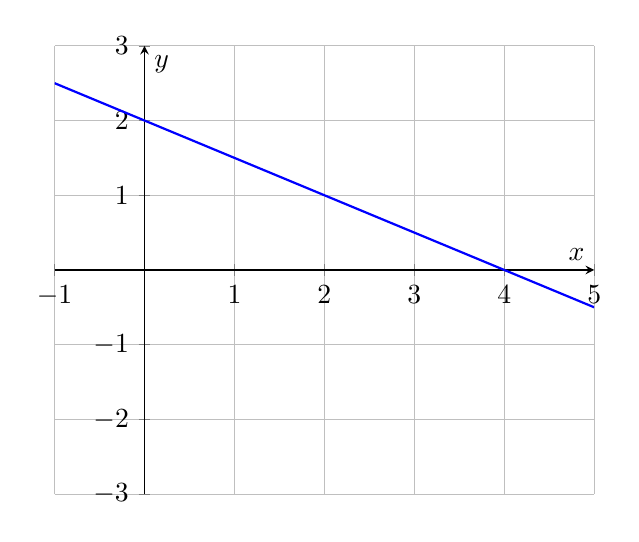
\begin{tikzpicture}
					\begin{axis}[
						axis lines = middle,
						xlabel = {$x$},
						ylabel = {$y$},
						xmin = -1, xmax = 5,
						ymin = -3, ymax = 3,
						xtick={-1,0,1,2,3,4,5},
						ytick={-3,-2,-1,0,1,2,3},
						grid = both
						]
						
						% f(x) = -1/2 x + 2
						\addplot[
						domain=-1:5,
						samples=100,
						blue,
						thick
						] {-0.5*x + 2};
						
					\end{axis}
				\end{tikzpicture}
				
			\end{solution}
			\item $f(x)=-\dfrac{1}{2x}+2$
			
			\begin{solution}
				Not linear.
			\end{solution}
			\item $f(x)=(x+2)^2-(x-2)^2$
		
			\begin{solution}
				Simplifying, we get $f(x)=(x^2+4x+4)-(x^2-4x+4)=8x$, so the function is linear.
				
				To find the $x$-intercept, we need to solve the equation $8x=0$. Solving the equation, we get $x=0$, so the $x$-intercept is $(0,0)$.
				
				To find the $y$-intercept, set $x=0$. We get $y=0$, so the $y$-intercept is $(0,0)$. 
				
				Since the slope $m=8>0$, the function is increasing, and hence, has no minimum/maximum.
				
				To find the $x$ for which the function is positive/negative, we need to solve the inequalities $f(x)>0$ and $f(x)<0$. Note that it is enough to solve one of them.
				$$f(x)>0$$
				$$8x>0$$
				$$x>0.$$
				
				Therefore, the function is negative on $(-\infty,0)$ and positive on $(0,\infty)$.
				
				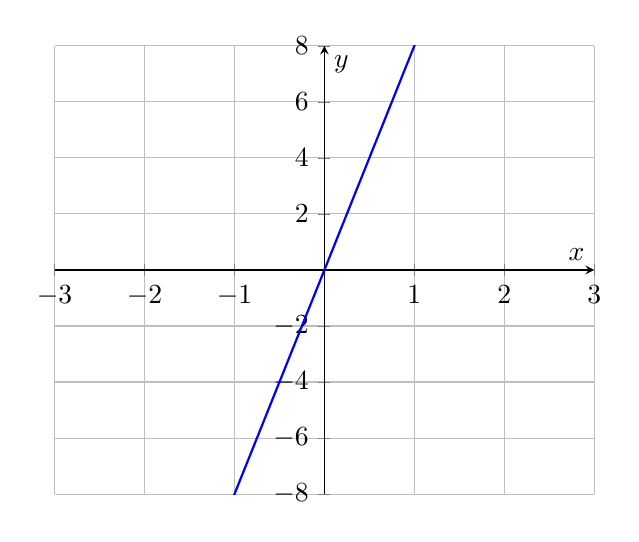
\begin{tikzpicture}
					\begin{axis}[
						axis lines = middle,
						xlabel = {$x$},
						ylabel = {$y$},
						xmin = -3, xmax = 3,
						ymin = -8, ymax = 8,
						xtick={-3,-2,-1,0,1,2,3},
						ytick={-8,-6,-4,-2,0,2,4,6,8},
						grid = both
						]
						
						% f(x) = 8x
						\addplot[
						domain=-3:3,
						samples=100,
						blue,
						thick
						] {8*x};
						
					\end{axis}
				\end{tikzpicture}
			\end{solution}
			\item $f(x)=-(x+1)(x-3)+x(x-2)$
			
			\begin{solution}
				Simplifying, we get $f(x)=-(x^2-3x+x-3)+(x^2-2x)=-x^2+2x+3+x^2-2x=3$, so the function is constant and, therefore, linear.
				
				There is no $x$-intercept and the $y$-intercept is $(0,3)$. 
				
				Since the function is constant, it is not increasing nor decreasing, and both the minimum and maximum are $3$, achieved at every $x\in\mathbb{R}$.
				
				Since $f(x)=3>0$, the function is positive for all $x\in\mathbb{R}$.
				
				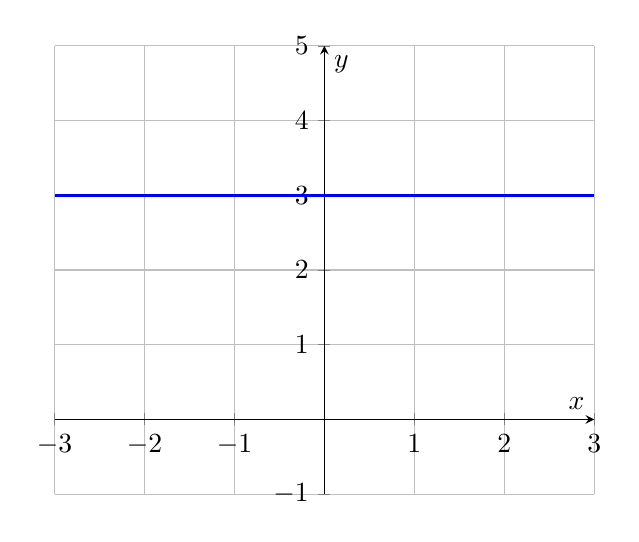
\begin{tikzpicture}
					\begin{axis}[
						axis lines = middle,
						xlabel = {$x$},
						ylabel = {$y$},
						xmin = -3, xmax = 3,
						ymin = -1, ymax = 5,
						xtick={-3,-2,-1,0,1,2,3},
						ytick={-1,0,1,2,3,4,5},
						grid = both
						]
						
						% f(x) = 3
						\addplot[
						domain=-3:3,
						blue,
						very thick
						] {3};
						
					\end{axis}
				\end{tikzpicture}
			\end{solution}
			\item $f(x)=\dfrac{x^2-1}{x-1}$
		
			\begin{solution}
				Not linear, the domain of this function is $\mathbb{R} \setminus\{1\}$, and the domain of all linear functions is an interval. (Even though when you simplify the expression algebraically, you get $\dfrac{(x-1)(x+1)}{x-1}=x+1$.)
			\end{solution}
		\end{enumerate}
		
		\item Solve the following equations.
		\begin{enumerate}
			\item $x^2-5x-14=0$
			\begin{solution}
				Use the quadratic formula.
				$$x_{1/2}=\dfrac{5\pm\sqrt{25+4\cdot 14}}{2}=\dfrac{5\pm\sqrt{81}}{2}=\dfrac{5\pm9}{2}.$$
				Thus, $x_1=\dfrac{5-9}{2}=-2$ and $x_2=\dfrac{5+9}{2}=7$.
			\end{solution}
			\item $x^2=x$
			\begin{solution}
				\begin{align*}
					x^2-x&=0\\
					x(x-1)&=0\\
					x=0 \text{ or } &x=1.
				\end{align*}
			\end{solution}
			\item $x^2=3x-5$
			\begin{solution}
				The equation is equivalent to $x^2-3x+5=0$. Since the discriminant is $D=(-3)^2-4\cdot 5=9-20=-11<0$, the equation has no real solutions.
			\end{solution}
			\item $x^2-x+(x+\dfrac{1}{2})^2=8\dfrac{1}{4}$
			\begin{solution}
				$$x^2-x+(x+\dfrac{1}{2})^2=8\dfrac{1}{4}$$
				$$x^2-x+x^2+x+\dfrac{1}{4}=8\dfrac{1}{4}$$
				$$2x^2=8$$
				$$x^2=4$$
				$$x_{1/2}=\pm2.$$
			\end{solution}
			\item $(3x-2)-(x-3)^2=-11$
			\begin{solution}
				$$(3x-2)-(x-3)^2=-11$$
				$$3x-2-(x^2-6x+9)=-11$$
				$$3x-2-x^2+6x-9+11=0$$
				$$-x^2+9x=0$$
				$$x(-x+9)=0$$
				$$x=0 \text{ or } x=9.$$
			\end{solution}
			\item $x+\dfrac{1}{x}=5,\ x\neq 0$
			\begin{solution}
				$$x+\dfrac{1}{x}=5$$
				$$x^2+1=5x$$
				$$x^2-5x+1=0$$
				$$x_{1/2}=\dfrac{5\pm\sqrt{25-4}}{2}$$
				$$x_{1/2}=\dfrac{5\pm \sqrt{21}}{2}.$$
			\end{solution}
			\item $\dfrac{x+1}{x-1}=3-\dfrac{x-2}{x+2},\ x\neq1,x\neq-2$
			\begin{solution}
				$$\dfrac{x+1}{x-1}=3-\dfrac{x-2}{x+2}$$
				$$(x+1)(x+2)=3(x-1)(x+2)-(x-2)(x-1)$$
				$$x^2+x+2x+2=3(x^2-x+2x-2)-(x^2-2x-x+2)$$
				$$x^2+3x+2=3x^2+3x-6-x^2+3x-2$$
				$$-x^2-3x+10=0$$
				$$x^2+3x-10=0$$
				$$x_{1/2}=\dfrac{-3\pm\sqrt{9+40}}{2}=\dfrac{-3\pm7}{2}.$$
				Hence, the solutions are $x_1=\dfrac{-3-7}{2}=-5$ and $x_2=\dfrac{-3+7}{2}=2$.
			\end{solution}
		\end{enumerate}
		
		\item Determine which of the following functions are quadratic. For those that are:
		\begin{itemize}
			\item Find the vertex form.
			\item Find the domain and range.
			\item Find the $x$ and $y$-intercepts (if any).
			\item Find the intervals of monotonicity.
			\item Find the minimum/maximum (if any).
			\item Sketch the graph of the function by sketching the $x$ and $y$-intercepts and the vertex.
		\end{itemize}
		\begin{enumerate}
			\item $f(x)=2-3x+x^2$
			
			\begin{solution}
				The function is quadratic. To find the vertex form, we complete the square in the following way
				\begin{align*}
					x^2-3x+2&=x^2-3x+\left(\dfrac{-3}{2}\right)^2-\left(\dfrac{-3}{2}\right)^2+2\\&= \left(x-\dfrac{3}{2}\right)^2-\dfrac{9}{4}+2\\
					&=\left(x-\dfrac{3}{2}\right)^2-\dfrac{1}{4}
				\end{align*}
				
				The domain of any quadratic function is $\mathbb{R}$, and the range is $\left[-\dfrac{1}{4},\infty \right).$
				
				To find the $x$-intercepts, we solve the equation $x^2-3x+2=0$, which is equivalent to $(x-1)(x-2)=0$, i.e., $x=1, x=2$. Thus, the function has two $x$-intercepts $(1,0)$ and $(2,0)$. To find the $y$-intercept, we set $x=0$ i.e. $0^2-3\cdot 0+2=2$, so the $y$-intercept is $(0,2)$.
				
				The function is decreasing on $(-\infty,\dfrac{3}{2})$ and it is increasing on $(\dfrac{3}{2},\infty)$.
				
				The function has a minimum at the point $\left(\dfrac{3}{2},-\dfrac{1}{4}\right)$ and has no maximum.
				
				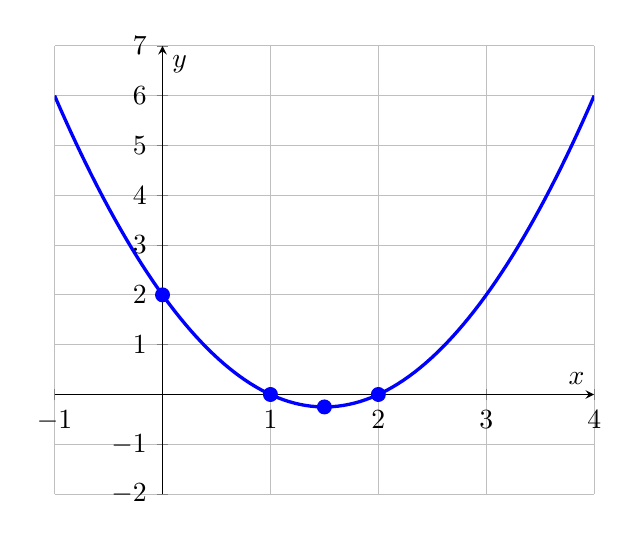
\begin{tikzpicture}
					\begin{axis}[
						axis lines = middle,
						xlabel = {$x$},
						ylabel = {$y$},
						xmin = -1, xmax = 4,
						ymin = -2, ymax = 7,
						xtick={-1,0,1,2,3,4},
						ytick={-2,-1,0,1,2,3,4,5,6,7},
						grid = both
						]
						
						% f(x) = x^2 - 3x + 2
						\addplot[
						domain=-1:4,
						samples=100,
						blue,
						very thick
						] {x^2 - 3*x + 2};
						
						% x-intercepts: (1,0) and (2,0)
						\addplot[
						only marks,
						mark=*,
						mark size=2.5pt,
						blue
						] coordinates {(1,0) (2,0)};
						
						% y-intercept: (0,2)
						\addplot[
						only marks,
						mark=*,
						mark size=2.5pt,
						blue
						] coordinates {(0,2)};
						
						% Vertex: (1.5,-1/4)
						\addplot[
						only marks,
						mark=*,
						mark size=2.5pt,
						blue
						] coordinates {(1.5,-0.25)};
						
					\end{axis}
				\end{tikzpicture}
			\end{solution}
			\item $f(x)=(x+2)^2-(x-2)^2$
			
			\begin{solution}
				Simplifying, we get $f(x)=(x^2+4x+4)-(x^2-4x+4)=8x$, so the function is not quadratic (it is linear).
			\end{solution}
			\item $f(x)=\dfrac{x^2-1}{x-1}$
			
			\begin{solution}
				Not quadratic (it is a rational function).
			\end{solution}
			\item $f(x)=3x-(x+\dfrac{3}{2})^2$
			
			\begin{solution}
				Simplifying, we get $f(x)=3x-(x^2+3x+\dfrac{9}{4})=-x^2-\dfrac{9}{4}$, so the function is quadratic. The vertex form of the function is $f(x)=-(x-0)^2-\dfrac{9}{4}$.
				
				The domain of any quadratic function is $\mathbb{R}$, and the range is $\left( -\infty, -\dfrac{9}{4}\right]$.
				
				To find the $x$-intercept, we solve the equation $-x^2-\dfrac{9}{4}=0$, which is equivalent to $x^2=-\dfrac{9}{4}$. But this equation has no solutions and therefore there are no $x$-intercepts. To find the $y$-intercept, we set $x=0$ i.e. $-0^2-\dfrac{9}{4}=-\dfrac{9}{4}$, so the $y$-intercept is $(0,-\dfrac{9}{4})$.
				
				The function is increasing on $(-\infty,0)$ and it is decreasing on $(0,\infty)$.
				
				The function has a maximum at the point $\left(0,-\dfrac{9}{4}\right)$ and has no minimum.
				
				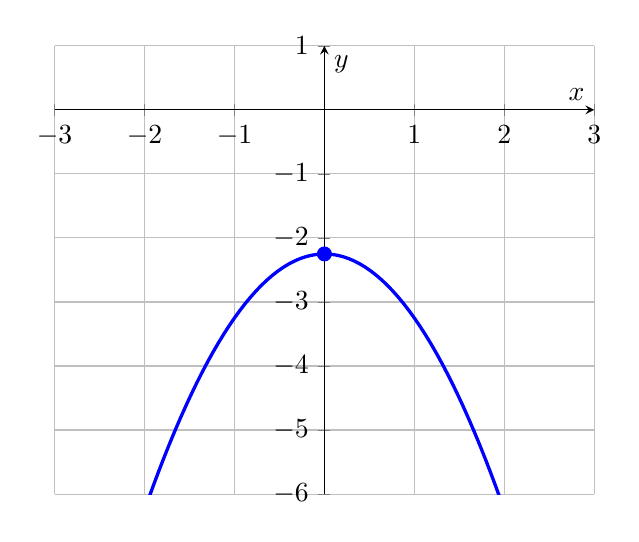
\begin{tikzpicture}
					\begin{axis}[
						axis lines = middle,
						xlabel = {$x$},
						ylabel = {$y$},
						xmin = -3, xmax = 3,
						ymin = -6, ymax = 1,
						xtick={-3,-2,-1,0,1,2,3},
						ytick={-6,-5,-4,-3,-2,-1,0,1},
						grid = both
						]
						
						% f(x) = 3x - (x + 3/2)^2
						\addplot[
						domain=-3:3,
						samples=100,
						blue,
						very thick
						] {3*x - (x + 1.5)^2};
						
						
						% Vertex: (0,-9/4)
						\addplot[
						only marks,
						mark=*,
						mark size=2.5pt,
						blue
						] coordinates {(0,-2.25)};
						
					\end{axis}
				\end{tikzpicture}
			\end{solution}
			\item $f(x)=(x+1)^3-(x+1)(x^2-x+1)$
	
			\begin{solution}
				Simplifying, we get $f(x)=(x^3+3x^2+3x+1)-(x^3+1)=3x^2+3x$, so the function is quadratic.
				
				To find the vertex form, we complete the square in the following way
				\begin{align*}
					3x^2+3x&=3(x^2+x)\\
					&=3(x^2+x+\left(\dfrac{1}{2}\right)^2-\left(\dfrac{1}{2}\right)^2)\\
					&=3(\left(x+\dfrac{1}{2}\right)^2-\dfrac{1}{4})\\
					&=3\left(x+\dfrac{1}{2}\right)^2-\dfrac{3}{4}.
				\end{align*}
				
				The domain of any quadratic function is $\mathbb{R}$, and the range is $\left[-\dfrac{3}{4},\infty \right).$
				
				To find the $x$-intercept, we solve the equation $3x^2+3x=0$, which is equivalent to $3x(x+1)=0$, i.e., $x=0, x=-1$. Thus, the function has two $x$-intercepts $(-1,0)$ and $(0,0)$. To find the $y$-intercept, we set $x=0$ i.e. $3\cdot0^2+3\cdot 0=0$, so the $y$-intercept is $(0,0)$.
				
				The function is decreasing on $(-\infty,-\dfrac{1}{2})$ and it is increasing on $(-\dfrac{1}{2},\infty)$.
				
				The function has a minimum at the point $\left(-\dfrac{1}{2},-\dfrac{3}{4}\right)$ and has no maximum.
				
				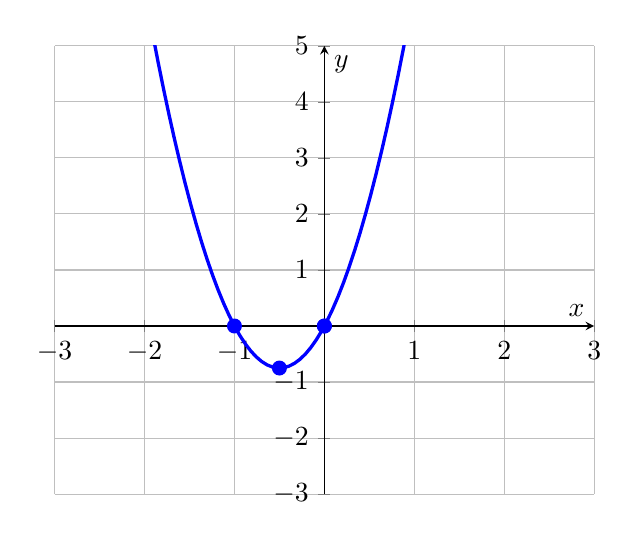
\begin{tikzpicture}
					\begin{axis}[
						axis lines = middle,
						xlabel = {$x$},
						ylabel = {$y$},
						xmin = -3, xmax = 3,
						ymin = -3, ymax = 5,
						xtick={-3,-2,-1,0,1,2,3},
						ytick={-3,-2,-1,0,1,2,3,4,5},
						grid = both
						]
						
						% f(x) = (x+1)^3 - (x+1)(x^2-x+1)
						% Simplified: f(x) = 3x^2 + 3x
						\addplot[
						domain=-3:3,
						samples=100,
						blue,
						very thick
						] {3*x^2 + 3*x};
						
						% x-intercepts: (-1,0) and (0,0)
						\addplot[
						only marks,
						mark=*,
						mark size=2.5pt,
						blue
						] coordinates {(-1,0) (0,0)};
						
						% y-intercept: (0,0)
						\addplot[
						only marks,
						mark=*,
						mark size=2.5pt,
						blue
						] coordinates {(0,0)};
						
						% Vertex: (-1/2,-3/4)
						\addplot[
						only marks,
						mark=*,
						mark size=2.5pt,
						blue
						] coordinates {(-0.5,-0.75)};
						
					\end{axis}
				\end{tikzpicture}
			\end{solution}	
		\end{enumerate}
		
		
		\item Find an equation for the line passing through the points $(1,2)$ and $(-1,0)$. Write your answer in the form $y=ax+b$.
		
		\begin{solution}
			The equation of a nonvertical line passing through two points $(x_1,y_1)$ and $(x_2,y_2)$ is $y-y_1=m(x-x_1)$, where the slope $m=\dfrac{y_2-y_1}{x_2-x_1}$. Note that it does not matter which point is first and which is second - they form the same line. For the given line, the slope is $m=\dfrac{2-0}{1-(-1)}=1$, so the equation of the line is $y-2=1(x-1)$, or $y=x+1$.
		\end{solution}
		\item Find an equation for the line passing through the points $(1,-5)$ and $(1,1)$. Write your answer in the form $ax+by+c=0$.
		\begin{solution}
			Notice that if you try to find the slope using the formula from above, you will get division by $0$. This indicates a vertical line (draw a sketch to confirm this). Since the $x$-coordinate of the two points does not change and is $1$, the equation of the line is $x=1$, or $x-1=0$.
		\end{solution}
		\item Find an equation for the line with slope $-1$, passing through the point $(-2,2)$. Write your answer in the form $y=ax+b$.
		\begin{solution}
			The equation of the line is $y-2=-1(x-(-2))$, which simplified is $y=-x$.
		\end{solution}
		\item Find an equation for the line with $y$-intercept 3 and slope $-2$. Write your answer in the form $ax+by+c=0$.
		\begin{solution}
			If the line has $y$-intercept $3$, it passes through the point $(0,3)$. Hence, the equation of the line is $y-3=-2(x-0)$, or $2x+y-3=0$.
		\end{solution}
		\item Find an equation for the line parallel to $2x-3y=1$, passing through the point $(1,-1)$. Write your answer in the form $ax+by+c=0$.
		\begin{solution}
			Parallel lines have the same slope. To find the slope of the given line, write it in the form $y=\dfrac{2}{3}x-\dfrac{1}{3}$. This line has slope $2/3$, and hence, any line parallel to it has slope $2/3$. Thus, the equation of the line is $y-(-1)=\dfrac{2}{3}(x-1)$, or $2x-3y-5=0$.
		\end{solution}
		\item Let $l_1$ be the line that passes through the points $(1,2)$ and $(-1,3)$. Find an equation for the line that is parallel to $l_1$ with $x$-intercept 2. Write your answer in the form $ax+by+c=0$.
		\begin{solution}
			The line is parallel to $l_1$, so it has the same slope $m=\dfrac{-1-1}{3-2}=-2$, and passes through the point $(2,0)$. Hence, its equation is $y-0=-2(x-2)$, or $2x+y-4=0$.
		\end{solution}
		\item Find the value of $k$ for which the line $2x-ky=1$
		\begin{enumerate}
			\item passes through the point $(1,-2)$.
			\begin{solution}
				If a line passes through a point, then the coordinates of the point satisfy the equation of the line. Hence, we have $2\cdot1-k\cdot(-2)=1$. Solving for $k$, we get $k=-\dfrac{1}{2}$.
			\end{solution}
			\item passes through the point $(1,0)$.
			\begin{solution}
				Similarly to part (a), we have $2\cdot 1-k\cdot 0=1$, or $2=1$. This equation does not have any solutions ($2=1$ is not a true statement for any $x$), so there is no $k$ that satisfies this condition.
			\end{solution}
			\item passes through the point $(\dfrac{1}{2},0)$.
			\begin{solution}
				In this case, we get the equation $2\cdot\dfrac{1}{2}-k\cdot0=1$, or $1=1$. Any real number $k \in \mathbb{R}$ satisfies this equation.
			\end{solution}
			\item is parallel to the line $2x+y=1$.
			\begin{solution}
				Transforming the equations to the form $y=mx+b$, we notice that the slope of the line $2x+y=1$ is $-2$ and the slope of the line $2x-ky=1$ is $\dfrac{2}{k}$ whenever $k\neq0$. Since the lines are parallel, the slopes are equal $-2=\dfrac{2}{k}$ and hence $k=-1$.
			\end{solution}
			\item is perpendicular to the line $2x+y=1$.
			\begin{solution}
				If two lines with slopes $m_1\neq 0$ and $m_2\neq 0$ are perpendicular, then $m_1\cdot m_2=-1$. The slope of $2x+y=1$ is $-2$ and hence $-2\cdot\dfrac{2}{k}=-1$. Solving this equation, we get $k=4$.
			\end{solution}
			\item is parallel to the line passing through the points $(1,-1)$ and $(3,-2)$.
			\begin{solution}
				The slope of this line is $m=\dfrac{-2-(-1)}{3-1}=-\dfrac{1}{2}$. Hence, $-\dfrac{1}{2}=\dfrac{2}{k}$ and $k=-4$.
			\end{solution}
			\item is perpendicular to the line $y=2$.
			\begin{solution}
				Since this line has slope $0$, we cannot use the equation from part (e). However, lines with slope $0$ are horizontal, so any line perpendicular to it has to be vertical. Thus, we need to find a $k$ for which $2x-ky=1$ is vertical. This happens when $k=0$.
			\end{solution}
			\item whose nonzero coordinates of the $x$- and $y$-intercepts are equal.
			\begin{solution}
				The $x$-intercept is obtained by setting $y=0$. Hence, $2x=1$ and $x=\dfrac{1}{2}$. The $y$-intercept is obtained by setting $x=0$. Hence, $-ky=1$ and $y=-\dfrac{1}{k}$, provided $k\neq 0$ (note that when $k=0$, the line is horizontal so it has no $y$-intercept). 
				
				Since the intercepts are equal, we set $\dfrac{1}{2}=-\dfrac{1}{k}$, so $k=-2$.
			\end{solution}
	\end{enumerate}
			\item The bisector of a line segment is a line that passes through the midpoint of the line segment and is perpendicular to it. Find an equation of the bisector of the line segment that connects the points $(-3,-5)$ and $(1,1)$. Write the equation in the form $y=ax+b$.
			\begin{solution}
				The midpoint of the line segment has coordinates $\left(\dfrac{-3+1}{2},\dfrac{-5+1}{2}\right)=(-1,-2)$. Since the bisector is perpendicular to the line segment, $m_1\cdot m_2=-1$ holds for their respective slopes. The slope of the line segment is $m_1=\dfrac{1-(-5)}{1-(-3)}=\dfrac{3}{2}$. Therefore, we find the slope $m_2$ of the line by solving the equation $\dfrac{3}{2}\cdot m_2=-1$. Hence, $m_2=-\dfrac{2}{3}$, so the equation of the line is $y-(-2)=-\dfrac{2}{3}(x-(-1))$, or $y=-\dfrac{2}{3}x-\dfrac{8}{3}$.
			\end{solution}
	
		
		\item Determine whether the following statements are true or false. Justify your reasoning.
		\begin{enumerate}
			\item If a linear function has a negative $x$-intercept and a positive $y$-intercept, then its slope must be positive.
			\begin{solution}
				True. Say the $x$-intercept is $(a,0)$ and the $y$-intercept is $(0,b)$. Then the slope is $-b/a$, which is positive since $a$ is negative and $b$ is positive.
			\end{solution}
			\item If $f(x)=ax+b$ and $f(3)=f(7)$, then the graph of $f(x)$ is a horizontal line.
			\begin{solution}
				True. $f(3)=3a+b$ and $f(7)=7a+b$, which means $3a+b=7a+b \iff -4a=0 \iff a=0$. If the slope is 0, then the line is horizontal.
			\end{solution}
			\item If a quadratic function has a negative leading coefficient, then it has to have $x$-intercepts.
			\begin{solution}
				False. The graph of a quadratic function with a negative leading coefficient is open downwards, but the whole graph can be below the $x$-axis and therefore, have no $x$-intercepts. See for example the following function.
				
				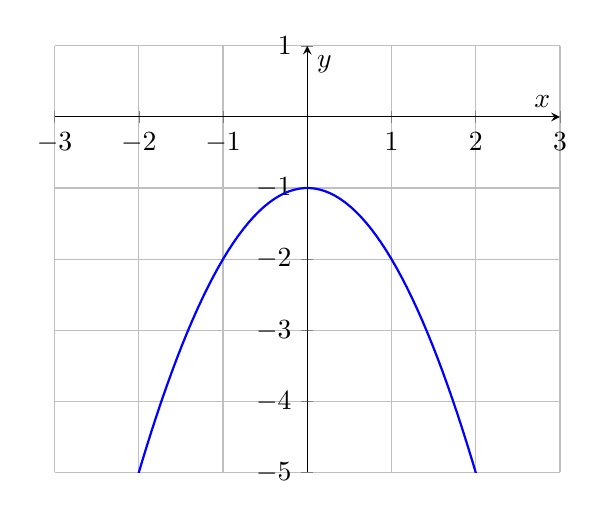
\begin{tikzpicture}
					\begin{axis}[
						axis lines=middle,
						xmin=-3, xmax=3,
						ymin=-5, ymax=1,
						xtick={-3,-2,-1,0,1,2,3},
						ytick={-5,-4,-3,-2,-1,0,1},
						grid=both,
						minor tick num=0,
						xlabel={$x$},
						ylabel={$y$},
						width=8cm,
						height=7cm,
						]
						\addplot[
						domain=-3:3,
						samples=100,
						thick,
						blue,
						] {-x^2-1};
					\end{axis}
				\end{tikzpicture}
			\end{solution}
			\item The function $f(x)=-2(x-3)^2+8$ has a minimum at $(3,8)$.
			\begin{solution}
				False. The vertex form implies that the vertex is at $(3,8)$, however, the leading coefficient is $-2<0$, so the function has a maximum and not a minimum.
			\end{solution}
			\item There exist two perpendicular lines with positive slopes.
			\begin{solution}
				False. If the lines have slopes $m_1, m_2$, then $m_1\cdot m_2=-1$, which is not possible if both $m_1$ and $m_2$ are positive.
			\end{solution}
			\item A vertical line has slope 0.
			\begin{solution}
				False. The slope of a line is only defined for non-vertical lines.
			\end{solution}
			\item The lines $ax+y=b$ and $ax-y=b$ are perpendicular for every $a\in\mathbb{R}\setminus\{0\}$.
			\begin{solution}
				False. The first line has slope $-a$ and the second line has slope $a$. If the lines are perpendicular, then $-a\cdot a=-1$, which is true only for $a=\pm1$ and not for all nonzero real numbers.
			\end{solution}
			\item The lines $ax+y=b$ and $x-ay=b$ are perpendicular for every positive real number $a$.
			\begin{solution}
				True. The slope of the first line is $-a$ and the slope of the second line is $1/a$ (note that we have no issues with $a=0$ since $a$ is positive). Then $-a\cdot \dfrac{1}{a}=-1$, so the lines are perpendicular.
			\end{solution}
		\end{enumerate}
		
	\end{enumerate}
	
	\newpage
	
	\section{Algebraic Functions}
	\begin{enumerate}
		
		\item Find the implied domain of the following power functions.
		\begin{enumerate}
			\item $f_1(x)=\sqrt{2}x^{2/3}$
			\begin{solution}
				The domain is $\mathbb{R}$.
			\end{solution}
			\item $f_2(x)=-3x^{-3}$
			\begin{solution}
				The domain is $\mathbb{R}\setminus \{0\}$
			\end{solution}
			\item $f_3(x)=2x^{-5/2}$
			\begin{solution}
				The domain is $(0,\infty)$.
			\end{solution}
			\item $f_4(x)=\dfrac{x^{1/4}}{4}$
			\begin{solution}
				The domain is $[0,\infty)$.
			\end{solution}
		\end{enumerate}
		Then find $f_1(-8), f_2(-3), f_3(4), f_4(16)$.
		\begin{solution}
			$$f_1(-8)=\sqrt{2}(-8)^{2/3}=\sqrt{2}((-2)^3)^{2/3}=\sqrt{2} (-2)^2=4\sqrt{2}$$
			
			$$f_2(-3)=-3\cdot(-3)^{-3}=-3\cdot \dfrac{1}{(-3)^3}=-3\cdot \dfrac{1}{-27}=\dfrac{1}{9}$$
			
			$$f_3(4)=2\cdot 4^{-5/2}=2\cdot (2^2)^{-5/2}=2\cdot 2^{(-5)}=2^{-4}=\dfrac{1}{16}$$
			
			$$f_4(16)=\dfrac{16^{1/4}}{4}=\dfrac{(2^4)^{1/4}}{4}=\dfrac{2}{4}=\dfrac{1}{2}.$$
		\end{solution}
		
		\item Simplify the expression to one involving only positive exponents. Assume that everything is well-defined.
		\begin{enumerate}
			\item $\left(\dfrac{x^{-1/4}y}{xz^2}\right)^{-4}$
			\begin{solution}
				$\left(\dfrac{x^{-1/4}y}{xz^2}\right)^{-4}=\dfrac{(x^{-1/4})^{-4}y^{-4}}{x^{-4}(z^2)^{-4}}=\dfrac{xy^{-4}}{x^{-4}z^{-8}}=\dfrac{xx^4z^8}{y^4}=\dfrac{x^5z^8}{y^4}.$
			\end{solution}
			\item $\dfrac{(x^3y)^{-1}(8^{-1}x^4y^3)}{(2x^2y^{-3})^{-2}}$
			\begin{solution}
				$\dfrac{(x^3y)^{-1}(8^{-1}x^4y^3)}{(2x^2y^{-3})^{-2}}=\dfrac{x^{-3}y^{-1}8^{-1}x^4y^3}{2^{-2}x^{-4}y^6}=\dfrac{xy^28^{-1}}{2^{-2}x^{-4}y^6}=\dfrac{xx^42^2}{8y^{6-2}}=\dfrac{x^5}{2y^4}.$
			\end{solution}
		\end{enumerate}
		\item Let $n$ and $x$ be positive integers. Write the following expression $\dfrac{\sqrt[3]{x^{6n}x^{-3n-9}}}{\sqrt{x^{2(n+2)}}}$ in the form $x^k$, for some integer $k$. 
		\begin{solution}
			$\dfrac{\sqrt[3]{x^{6n}x^{-3n-9}}}{\sqrt{x^{2(n+2)}}}=\dfrac{x^{6n/3}x^{(-3n-9)/3}}{x^{2(n+2)/2}}=\dfrac{x^{2n}x^{-n-3}}{x^{n+2}}=\dfrac{x^{2n-n-3}}{x^{n+2}}=\dfrac{x^{n-3}}{x^{n+2}}=x^{(n-3)-(n+2)}=x^{-5}.$
		\end{solution}
		
		\item Determine the degree, leading coefficient, leading term and constant term of the following polynomials.
		\begin{enumerate}
			\item $-(1-x)^2+2(x-1)(2x+1)-(x-2)(x+2)$
			\begin{solution}
				\begin{align*}
					&-(1-x)^2+2(x-1)(2x+1)-(x-2)(x+2)\\&=-(1-2x+x^2)+2(2x^2+x-2x-1)-(x^2-4)\\
					&=-1+2x-x^2+4x^2+2x-4x-2-x^2+4\\
					&=2x^2+1
				\end{align*}
				The degree of the polynomial is 2, the leading coefficient is $2$, the leading term is $2x^2$ and the constant term is $1$.
			\end{solution}
			\item $(x-2)(x^2+2x+4)-(x-2)^3$
			\begin{solution}
				\begin{align*}
					&(x-2)(x^2+2x+4)-(x-2)^3\\
					&=(x^3-2^3)-(x^3-6x^2+12x-8)\\
					&=x^3-8-x^3+6x^2-12x+8\\
					&=6x^2-12x
				\end{align*}
				The degree of the polynomial is 2, the leading coefficient is 6, the leading term is $6x^2$ and the constant term is $0$.
			\end{solution}
			\item $(x^2+x-6)^2-2x(x+3)(x^2+1)$
			\begin{solution}
				\begin{align*}
					&(x^2+x-6)^2-2x(x+3)(x^2+1)\\
					&=(x^4+x^2+6^2+2x^3-12x^2-12x)-2x(x^3+x+3x^2+3)\\
					&=x^4+2x^3-11x^2-12x+36-2x^4-2x^2-6x^3-6x\\
					&=-x^4-4x^3-13x^2-18x+36
				\end{align*}
				The degree of the polynomial is 4, the leading coefficient is -1, the leading term is $-x^4$ and the constant term is 36.
			\end{solution}
		\end{enumerate}
		
		\item Determine the values of $a,b,c$ so that the polynomials $f(x)$ and $g(x)$ are equal.\begin{enumerate}
			\item 
			$
			f(x)=2(x-3)^2-4(x+1)
			$
			
			$
			g(x)=(a-1)x^2+(b+5)x+c.
			$
			
			\begin{solution}
				Two polynomials are equal if the corresponding coefficients are equal. We have
				$f(x)=2x^2-12x+18-4x-4=2x^2-16x+14$, so we get 
				$a-1=2, b+5=-16, c=14$, i.e. $a=3,b=-21,c=14$.
			\end{solution}
			
			\item $f(x)=(x-3)(2x^2-4x+5)+(x+2)(x^2-3x+1)$
			
			$g(x)=(a+b)x^3+(2a-c)x^2+(b+3c)x+11.
			$
			
			\begin{solution}
				We have $f(x)=2x^3-4x^2+5x-6x^2+12x-15+x^3-3x^2+x+2x^2-6x+2=3x^3-11x^2+12x-13$. Thus $a+b=3,2a-c=-11,b+3c=12$, i.e., $a=-\dfrac{24}{5},b=\dfrac{39}{5},c=\dfrac{7}{5}$.
			\end{solution}
		\end{enumerate}
		
		\item Find the (real) roots of the following polynomials.
		\begin{enumerate}
			\item $x^3-2x^2-x+2$
			\begin{solution}
				$x^3-2x^2-x+2=0 \iff x^2(x-2)-(x-2)=0\iff (x-2)(x^2-1)=0\iff (x-2)(x-1)(x+1)=0$ and therefore, the zeroes are $2,1,-1$.
			\end{solution}
			\item $x^3-4x^2+x+6$
			\begin{solution}
				This polynomial does not factor as easily as the previous one. Using the Integer Root theorem, the possible integer solutions to the equation $x^3-4x^2+x+6=0$ are the divisors of $6$, i.e., $\pm1,\pm2,\pm3,\pm6$. Notice that $-1$ is one solution. Then use long division of polynomials to divide the given polynomial by $x-(-1)=x+1$:
				
			$$
			\begin{array}{r@{}l}
				& \underline{x^2-5x+6} \\
				 x+1\,\big)\,& x^3-4x^2+x+6 \\[1mm]
				& \underline{x^3+x^2} \\[-1mm]
				& \phantom{x^3+}(-5x^2+x) \\[1mm]
				& \underline{\phantom{x^3+}(-5x^2-5x)} \\[-1mm]
				& \phantom{x^3-4x^2+}(6x+6) \\[1mm]
				& \underline{\phantom{x^3-4x^2+}(6x+6)} \\[-1mm]
				& 0
			\end{array}.
			$$
			Next, we solve the equation $x^2-5x+6=0\iff(x-3)(x-2)=0\iff x=3,x=2$.
			
			Thus, the roots of the polynomial are $-1,2,3$.
			\end{solution}
			\item $x^4+x^3+2x-4$
			\begin{solution}
				Similarly, we notice that 1 is a solution to the equation $x^4+x^3+2x-4=0$. We use long division to divide the given polynomial by $x-1$:
				
				$$
				\begin{array}{r@{}l}
					& \underline{x^3+2x^2+2x+4} \\
					x-1\,\big)\,& x^4+x^3+0x^2+2x-4 \\[1mm]
					& \underline{x^4-x^3} \\[-1mm]
					& \phantom{x^4+}(2x^3+0x^2) \\[1mm]
					& \underline{\phantom{x^4+}(2x^3-2x^2)} \\[-1mm]
					& \phantom{x^4+x^3+}(2x^2+2x) \\[1mm]
					& \underline{\phantom{x^4+x^3+}(2x^2-2x)} \\[-1mm]
					& \phantom{x^4+x^3+0x^2+}(4x-4) \\[1mm]
					& \underline{\phantom{x^4+x^3+0x^2+}(4x-4)} \\[-1mm]
					& 0
				\end{array}.
				$$
				
				Next, we solve the equation $x^3+2x^2+2x+4=0 \iff x^2(x+2)+2(x+2)=0\iff (x^2+2)(x+2)=0$. Since $x^2+2=0$ has no real solutions, the only roots of the polynomial are 1 and -2.
				
				Note that if $x^3+2x^2+2x+4=0$ was not easily factorizable, we would use the integer root theorem and long division, as previously. 
			\end{solution}
		\end{enumerate}
		
		\item Classify the following functions as one of the following: power functions, polynomial functions, rational functions, algebraic functions that are none of the previous types. Note that some functions belong to more than one function class.
		\begin{enumerate}
			\item $f(x)=\sqrt{x}$
			\begin{solution}
				Power function.
			\end{solution}
			\item $f(x)=\sqrt{\pi}$
			\begin{solution}
				Polynomial function, power function, rational function.
			\end{solution}
			\item $f(x)=x^2$
			\begin{solution}
				Polynomial function, power function, rational function.
			\end{solution}
			\item $f(x)=2(x^{3/2}+1)$
			\begin{solution}
				Algebraic function.
			\end{solution}
			\item $f(x)=2x^{5/2}-x^{3/2}+1$
			\begin{solution}
				Algebraic function.
			\end{solution}
			\item $f(x)=\dfrac{1+x}{1+x^2}$
			\begin{solution}
				Rational function.
			\end{solution}
			\item $f(x)=\dfrac{1+x}{1+\sqrt{x}}$
			\begin{solution}
				Algebraic function.
			\end{solution}
		\end{enumerate}
		
		
		
		\item Find the (implied) domain and the zeroes (if any) of the following functions.
		\begin{enumerate}
			\item $f(x)=x^2-x+2$
		
			\begin{solution}
				This is a polynomial function (quadratic, to be specific) and therefore, the domain is $\mathbb{R}$.
				
				To find the zeroes, we have to solve the equation $x^2-x+2=0$. However, this equation has no real solutions, so the function has no zeroes.
			\end{solution}
			\item $f(x)=\dfrac{x^2-x-2}{5}$
			\begin{solution}
				This is also a polynomial function and hence the domain is $\mathbb{R}$. 
				
				The zeroes are $-1$ and $2$, obtained by solving the equation $\dfrac{x^2-x-2}{5}=0$.
			\end{solution}
			\item $f(x)=\dfrac{x-2}{2x^2-3x+1}$
			\begin{solution}
				This is a rational function that is defined for all real numbers such that $2x^2-3x+1\neq0$. The solutions to this equation are $x=1/2$ and $x=1$ and hence, the domain of the function is $\mathbb{R} \setminus \{1,\dfrac{1}{2}\}$.
				
				$\dfrac{x-2}{2x^2-3x+1}=0$ whenever $x-2=0$ or $x=2$. Therefore, the function has one zero $2$. 
			\end{solution}
			\item $f(x)=\dfrac{x-2}{x^2-4}$
			\begin{solution}
				$x^2-4=0$ whenever $x=\pm 2$. Therefore, the domain of the function is $\mathbb{R}\setminus \{-2,2\}$.
				
				$\dfrac{x-2}{x^2-4}=0$ whenever $x-2=0$ or $x=2$. However, $2$ is not in the domain of the function, and therefore the function has no zeroes.
			\end{solution}
			\item $f(x)=\dfrac{x^2-1}{x^3-x^2+x-1}$
			\begin{solution}
				$$x^3-x^2+x-1=0$$
				$$x^2(x-1)+(x-1)=0$$
				$$(x-1)(x^2+1)=0$$
				$$x=1$$
				since $x^2+1\neq 0$ for any real number $x$. Therefore, the domain of the function is $\mathbb{R}\setminus \{1\}$.
				
				$x^2-1=0$ whenever $x^2=1$ i.e., whenever $x=\pm1$. However, $1$ is not in the domain of the function, and hence, the only zero of the function is $-1$.
			\end{solution}
			\item $f(x)=\dfrac{x^2+1}{x^3-2x+1}$
			\begin{solution}
				To find the domain, we need to solve the equation $x^3-2x+1=0$. First, notice that $x=1$ is a solution. Then, using long division, we conclude that $x^3-2x+1=(x-1)(x^2+x-1)$. Solving $x^2+x-1=0$, we get $x=\dfrac{-1\pm\sqrt{5}}{2}$. Thus the domain of the function is $\mathbb{R}\setminus \{1,\dfrac{-1\pm\sqrt{5}}{2}\}$.
				
				To find the zeroes, we need to solve $\dfrac{x^2+1}{x^3-2x+1}=0$, which is equivalent to $x^2+1=0$. This equation has no real solutions and hence, the function has no zeroes.
			\end{solution}
	
		\end{enumerate}
		
		\item Determine whether the following statements are true or false. Justify your reasoning.
		\begin{enumerate}
				\item If $f(x)=\sqrt{x-3}$, then the domain of $f$ is $[3,\infty)$.
				
				\item The function $f(x)=\sqrt[3]{x-5}$ has domain $[5,\infty)$.
				
				\item If $f(x)=\sqrt{(x-2)^2}$, then $f(x)=x-2$ for every $x$.
				
				\item The functions
				$$
				f(x)=\frac{x^2-4}{x-2}
				\qquad\text{and}\qquad
				g(x)=x+2
				$$
				are equal functions.
				
				\item The domain of
				$$
				f(x)=\frac{\sqrt{x-2}}{x-5}
				$$
				is $[2,5)\cup(5,\infty)$.
				\item The function $f(x)=x^{5/2}-x^{3/2}$ is a power function.
				\item The function $f(x)=\dfrac{x^3+x^2}{x}$ is a polynomial function.
				\item The function $f(x)=x^{5/3}$ is defined for every real number $x$.
				
				\setcounter{enumi}{3}
				\item The function $f(x)=x^{-2/3}$ is defined at $x=0$.
				
				\item The domain of $f(x)=(x-2)^{-1/2}$ is $(2,\infty)$.
				
				\item The function $f(x)=\sqrt[3]{x^2-4}$ is defined for every real number $x$.
				
				\setcounter{enumi}{8}
				\item Every polynomial function is an algebraic function.
				
				\setcounter{enumi}{14}
				\item If $x-3$ is a factor of $f(x)$, then $f(3)=0$.
				
				\setcounter{enumi}{16}
				\item The polynomial
				$$
				f(x)=x^4-16
				$$
				has exactly two real zeros.
				
				\setcounter{enumi}{25}
				\item If $f(x)=x^{2/3}$, then
				$$
				f(-8)=4.
				$$
				
				\item If $f(x)=x^{3/2}$, then
				$$
				f(-4)=-8.
				$$
		\end{enumerate}
		
		
	\end{enumerate}
	\newpage
		\section{Transformations and Symmetry}
	
	\begin{enumerate}
		\item The graph of the function $f(x)$ is given below. Sketch the graphs of the following functions and state the transformation of $f(x)$.
		\begin{enumerate}
			\item $f(x)+1, f(x)-1, f(x+1), f(x-1)$
			\item $2f(x), \dfrac{1}{2}f(x), f(2x), f(\dfrac{1}{2}x)$
			\item $-f(x),f(-x)$
		\end{enumerate}
		\item The graph of the function $f(x)$ is given below. Sketch the graphs of the following functions and explain which function transformations of $f(x)$  (and in what order) give $g(x)$. 
		\begin{enumerate}
			\item $g(x)=-2f(x-1)+1$
			\item $g(x)=$
			\item $g(x)=$
		\end{enumerate}
		\item Determine whether the given functions are even, odd, or neither.
	\end{enumerate}
	
		\section{Operations with Functions}
	
	\begin{enumerate}
		\item Let $f(x)=\dfrac{x}{x-2}$ and $g(x)=\dfrac{2x}{x-1}$. Find
		\begin{enumerate}
			\item $(f-g)(-2)$
			\begin{solution}
				$(f-g)(-2)=f(-2)-g(-2)=\dfrac{-2}{-2-2}-\dfrac{2(-2)}{-2-1}=\dfrac{1}{2}-\dfrac{4}{3}=-\dfrac{5}{6}$.
			\end{solution}
			\item $(f+g)(1)$
			\begin{solution}
				$g(x)$ is not defined for $x=1$, so $(f+g)(1)$ is undefined.
			\end{solution}
			\item $(f-g)(2)$
			\begin{solution}
				$f(x)$ is not defined for $x=2$, so $(f-g)(2)$ is undefined.
			\end{solution}
			\item $\dfrac{f}{g}(3)$
			\begin{solution}
				$\dfrac{f}{g}(3)=\dfrac{f(3)}{g(3)}=\dfrac{\dfrac{3}{3-2}}{\dfrac{2\cdot 3}{3-1}}=\dfrac{3}{3}=1$.
			\end{solution}
			\item $\dfrac{f}{g}(0)$
			\begin{solution}
				$g(0)=0$, so $\dfrac{f}{g}(0)$ is undefined.
			\end{solution}
			\item $g\cdot g(3)$
			\begin{solution}
				$g\cdot g(3)=g(3)\cdot g(3)=3\cdot 3=9.$
			\end{solution}
			\item $f\circ g(1)$
			\begin{solution}
				$f\circ g(1)=f(g(1))$, but $g$ is not defined at $1$, so $f\circ g(1)$ is undefined.
			\end{solution}
			\item $f\circ g(2)=f(g(2))=f\left(\dfrac{2\cdot 2}{2-1}\right)=f(4)=\dfrac{4}{4-2}=2$.
			\item $g \circ f(x)$
			\begin{solution}
				$g\circ f(x)=g(f(x))=g\left(\dfrac{x}{x-2}\right)=\dfrac{2\cdot\dfrac{x}{x-2}}{\dfrac{x}{x-2}-1}=\dfrac{\dfrac{2x}{x-2}}{\dfrac{2}{x-2}}\\=\dfrac{2x}{x-2}\cdot \dfrac{2}{x-2}=x$.
			\end{solution}
			\item $f \circ f (x)$
			\begin{solution}
				$f\circ f(x)=f(f(x))=f\left(\dfrac{x}{x-2}\right)=\dfrac{\dfrac{x}{x-2}}{\dfrac{x}{x-2}-2}=\dfrac{\dfrac{x}{x-2}}{\dfrac{-x+4}{x-2}}=\dfrac{x}{4-x}$.
			\end{solution}
		\end{enumerate}
		
		\item Use the table to find the indicated values or state that they cannot be determined based solely on the table. 
		
		\item Using the graphs of the function $f$ and $g$ below, find the following values or state they cannot be determined based on the image.
		
		\item Write the functions as a composition of at least three different functions. Note that there are several ways to do this, so the answer is not unique.
		\begin{enumerate}
			\item $f(x)=\dfrac{1}{\sqrt{x^2+1}}$
			\begin{solution}
				$f=f_1\circ f_2 \circ f_3$, where $f_1(x)=\dfrac{1}{x},f_2(x)=\sqrt{x},f_3(x)=x^2+1$
			\end{solution}
			\item $f(x)=3(x-1)^{3/2}$
			\begin{solution}
				$f=f_1\circ f_2 \circ f_3$, where $f_1(x)=3x,f_2(x)=x^{3/2},f_3(x)=x-1$
			\end{solution}
			\item $f(x)=\dfrac{\sqrt{(1+2x)^3}+2\sqrt{1+2x}-1-2x}{\sqrt{1+2x}}$
			\begin{solution}
				$f=f_1\circ f_2 \circ f_3$, where $f_1(x)=1+2x,f_2(x)=\sqrt{x},f_3(x)=\dfrac{x^3+2x-x^2}{x}$.
			\end{solution}
		\end{enumerate}
		
		\item Find the domain of the functions $f\circ g$, $g\circ f$, $f\circ f$, $g\circ g$, if
		\begin{enumerate}
			\item $f(x)=, g(x)=$
		\end{enumerate}
	\end{enumerate}
	
	
	\section{Solving Inequalities}
	
	\begin{enumerate}
		\item Find all the real values of $x$ that satisfy the following inequalities. Write your answer using interval notation or set builder notation.
		\begin{enumerate}
			\item $5x-3>2x+1$
			\begin{reading}
				Section: 1.8. 
				
				Subsection: Elementary inequality rules
			\end{reading}
			\begin{solution}
				\begin{align*}
					5x-3&>3x+1\\
					5x-2x&>1+3\\
					3x&>4\\
					x&>\dfrac{4}{3}
				\end{align*} 
				The solution is $\left(\dfrac{4}{3},\infty\right)$.
			\end{solution}
			\item $(x-2)^2\leq (x+1)^2$
				\begin{reading}
					Section: 1.8. 
					
					Subsection: Elementary inequality rules
				\end{reading}
				
				\begin{solution}
					\begin{align*}
						(x-2)^2&\leq (x+1)^2\\
						x^2-4x+3 &\leq x^2+2x+1\\
						-4x-2x&\leq 1-4\\
						-6x &\leq -3\\
						x &\geq \dfrac{1}{2}
					\end{align*}
					
					The solution is $\left[\dfrac{1}{2},\infty\right]$.
				\end{solution}
			\item $x^2-4x+3\leq 0$
			
			\begin{reading}
				Section: 1.8. 
				
				Subsection: Sign diagram technique
			\end{reading}
			
			\begin{solution}
				We need to solve the inequality $x^2-4x+3\leq 0$. In other words, we need to find all $x$ such that $g(x) \geq 0$, where $g(x)=x^2-4x+3$. The first step is to find the domain of $g(x)$. The domain of $g(x)$ is $\mathbb{R}$. Next, we find the zeroes by solving the equation $g(x)=0$.
				
				\begin{align*}
					x^2-4x+3&=0\\
					(x-1)(x-3)&=0\\
					x=1 \text{ or } x&=3.
				\end{align*}
				
				Both $1$ and $3$ are in the domain of $g(x)$, so they are both zeroes. Using this information, we can draw a sign chart. 
				
				\[
				\begin{tikzpicture}[scale=1]
					\draw[->] (-5,0) -- (5,0);
					
					\draw (-2.5,0) node[circle,blue,fill,inner sep=2pt]{};
					\draw (1.5,0) node[circle,blue,fill,inner sep=2pt]{};
					%	\draw[blue, thick, fill=white] (0,0) circle (2.5pt);
					
					\node at (-2.5, .5) {1};
					\node at (1.5, .5) {3};
					%\node at (0, .5) {$0$};
					\node at (-5,.5) {$g\colon$};
					\node at (-3.5,.5) {$+$};
					\node at (-0.4,.5) {$-$};
					\node at (3, .5) {$+$};
				\end{tikzpicture}
				\]
				
				Since we are trying to find all $x$ such that $x^2-4x+3$ is negative or equal to $0$, using the sign chart, the solution is $[1.3]$.
				
			\end{solution}
			\item $x(x-1)>(x-\dfrac{1}{2})^2$
			\begin{reading}
				Section: 1.8. 
				
				Subsection: Sign diagram technique
			\end{reading}
			
			\begin{solution}
				\begin{align*}
					x(x-1)&>(x-1\dfrac{1}{2})^2\\
					x^2-x&>x^2-x+\dfrac{1}{4}\\
					0&>\dfrac{1}{4}.
				\end{align*}
				
				Since $0>\dfrac{1}{4}$ is false for any $x$, there is no real solution to this inequality. We say that the solution is $\emptyset$ (the \textit{empty set}).
			\end{solution}
			\item $3x^2+5x+7>0$
			\begin{reading}
				Section: 1.8. 
				
				Subsection: Sign diagram technique
			\end{reading}
			
			\begin{solution}
				We need to solve the inequality $3x^2+5x+7> 0$. In other words, we need to find all $x$ such that $g(x) \geq 0$, where $g(x)=3x^2+5x+7$. However, this equation has no real solutions, so $g(x)$ is either positive everywhere or negative everywhere. We notice that for all $x$, $g(x)>0$. Hence, all real numbers satisfy this inequality, so the solution is $(-\infty,\infty)=\mathbb{R}$.
			\end{solution}
			\item $3x^2+5x+7\leq 0$
			\begin{reading}
				Section: 1.8. 
				
				Subsection: Sign diagram technique
			\end{reading}
			
			\begin{solution}
				From the previous exercise, we notice there are no $x$ such that $3x^2+5x+7\leq 0$, so the solution is $\emptyset$.
			\end{solution}
			\item $\dfrac{2x-1}{x+2}\geq 0$
			\begin{reading}
				Section: 1.8. 
				
				Subsection: Sign diagram technique
			\end{reading}
			
			\begin{solution}
				We need to solve the inequality $\dfrac{2x-1}{x+2}\geq 0$. In other words, we need to find all $x$ such that $g(x) \geq 0$, where $g(x)=\dfrac{2x-1}{x+2}$. The first step is to find the domain of $g(x)$, which is all real numbers such that $x+2\neq0$. Thus, the domain of $g(x)$ is $(-\infty, -2) \cup (-2, \infty) $. Next, we find the zeroes by solving the equation $g(x)=0$.
				
				\begin{align*}
					\dfrac{2x-1}{x+2}&=0\\
					2x-1&=0\\
					x&=\dfrac{1}{2}.
				\end{align*}
				
				$\dfrac{1}{2}$ is in the domain of $g(x)$, so it is a zero. Using this information, we can draw a sign chart. 
				
				\[
				\begin{tikzpicture}[scale=1]
					\draw[->] (-5,0) -- (5,0);
					
					%\draw (-2.5,0) node[circle,blue,fill,inner sep=2pt]{};
					\draw (1.5,0) node[circle,blue,fill,inner sep=2pt]{};
					\draw[blue, thick, fill=white] (-2.5,0) circle (2.5pt);
					
					\node at (-2.5, .5) {-2};
					\node at (1.5, .5) {1/2};
					%\node at (0, .5) {$0$};
					\node at (-5,.5) {$g\colon$};
					\node at (-3.5,.5) {$+$};
					\node at (-0.4,.5) {$-$};
					\node at (3, .5) {$+$};
				\end{tikzpicture}
				\]		
				
				Since we are trying to find all $x$ such that $\dfrac{2x-1}{x+2}$ is positive or equal to $0$, using the sign chart, we conclude that the solution is $(\infty, -2) \cup [1/2, \infty]$.
			\end{solution}
			\item $\dfrac{2x-1}{x+2} \geq 2$
			\begin{reading}
				Section: 1.8. 
				
				Subsection: Sign diagram technique
			\end{reading}
			
			\begin{solution}
				\begin{align*}
					\dfrac{2x-1}{x+2}&\geq 2\\
					\dfrac{2x-1}{x+2} - 2&\geq 0\\
					\dfrac{2x-1-2x-4}{x+2} &\geq 0\\
					\dfrac{-5}{x+2}&\geq 0
				\end{align*}
				
				We need to solve the inequality $\dfrac{-5}{x+2}\geq 0$. In other words, we need to find all $x$ such that $g(x) \geq 0$, where $g(x)=\dfrac{-5}{x+2}$. The first step is to find the domain of $g(x)$. The domain of $g(x)$ is $(-\infty, -2) \cup (-2, \infty) $. Next, we find the zeroes by solving the equation $g(x)=0$.
				\begin{align*}
					\dfrac{-5}{x+2}&=0\\
					-5&=0
				\end{align*}
				
				so this equation has no solutions, and hence $g(x)$ has no zeroes. This does NOT mean we cannot solve the inequality. 
				
				We can still draw a sign chart. 
				
				\[
				\begin{tikzpicture}[scale=1]
					\draw[->] (-4,0) -- (0,0);
					
					%\draw (-2.5,0) node[circle,blue,fill,inner sep=2pt]{};
					%\draw (1.5,0) node[circle,blue,fill,inner sep=2pt]{};
					\draw[blue, thick, fill=white] (-2,0) circle (2.5pt);
					
					\node at (-2, .5) {-2};
					%	\node at (1.5, .5) {1/2};
					%\node at (0, .5) {$0$};
					\node at (-5,.5) {$g\colon$};
					\node at (-3.5,.5) {$+$};
					\node at (-0.5,.5) {$-$};
					%	\node at (3, .5) {$+$};
				\end{tikzpicture}
				\]		
				
				Since we are trying to find all $x$ such that $\dfrac{-5}{x+2}$ is positive or equal to $0$, using the sign chart, we conclude that the solution is $(-\infty,-2)$.
			\end{solution}
			\item $(x+1)(2x-1)^2(2-x)<0$
			\begin{reading}
				Section: 1.8. 
				
				Subsection: Sign diagram technique
			\end{reading}
			
			\begin{solution}
					We need to solve the inequality $(x+1)(2x-1)^2(2-x)< 0$. In other words, we need to find all $x$ such that $g(x) < 0$, where $g(x)=(x+1)(2x-1)^2(2-x)$. The first step is to find the domain of $g(x)$. The domain of $g(x)$ is $\mathbb{R}$. Next, we find the zeroes by solving the equation $(x+1)(2x-1)^2(2-x)=0$. The solutions are $x=-1,x=\dfrac{1}{2},x=2$ and all three solutions are in the domain.
				We draw a sign chart. 
				
				\[
				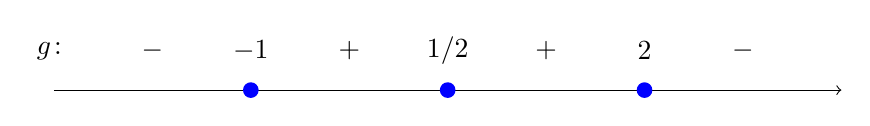
\begin{tikzpicture}[scale=1]
					\draw[->] (-7,0) -- (3,0);
					
					\draw (-2,0) node[circle,blue,fill,inner sep=2pt]{};
					\draw (-4.5,0) node[circle,blue,fill,inner sep=2pt]{};
					\draw (0.5,0) node[circle,blue,fill,inner sep=2pt]{};
					%\draw[blue, thick, fill=white] (-2,0) circle (2.5pt);
					
					\node at (-2, .5) {1/2};
					\node at (-4.5, .5) {$-1$};
					\node at (0.5, .5) {2};
					\node at (-7,.5) {$g\colon$};
					\node at (-3.25,.5) {$+$};
					\node at (-0.75,.5) {$+$};
					\node at (1.75, .5) {$-$};
					\node at (-5.75, .5) {$-$};
				\end{tikzpicture}
				\]		
				
				Since we are trying to find all $x$ such that $(x+1)(2x-1)^2(2-x)$ is negative, using the sign chart, we conclude that the solution is $(-\infty,-1)\cup (2,\infty)$.
				\end{solution}

			\item $\dfrac{(x+1)(2x-1)^2}{2-x}\leq 0$
			\begin{reading}
				Section: 1.8. 
				
				Subsection: Sign diagram technique
			\end{reading}
			
				\begin{solution}
				We need to solve the inequality $\dfrac{(x+1)(2x-1)^2}{2-x}\leq 0$. In other words, we need to find all $x$ such that $g(x) \leq 0$, where $g(x)=\dfrac{(x+1)(2x-1)^2}{2-x}$. The first step is to find the domain of $g(x)$. The domain of $g(x)$ is $\mathbb{R}\setminus \{2\}$. Next, we find the zeroes by solving the equation $\dfrac{(x+1)(2x-1)^2}{2-x}=0$. The solutions are $x=-1,x=\dfrac{1}{2}$ and both are in the domain.
				We draw a sign chart. 
				
				\[
				\begin{tikzpicture}[scale=1]
					\draw[->] (-7,0) -- (3,0);
					
					\draw (-2,0) node[circle,blue,fill,inner sep=2pt]{};
					\draw (-4.5,0) node[circle,blue,fill,inner sep=2pt]{};
					%\draw (0.5,0) node[circle,blue,fill,inner sep=2pt]{};
					\draw[blue, thick, fill=white] (0.5,0) circle (2.5pt);
					
					\node at (-2, .5) {1/2};
					\node at (-4.5, .5) {$-1$};
					\node at (0.5, .5) {2};
					\node at (-7,.5) {$g\colon$};
					\node at (-3.25,.5) {$+$};
					\node at (-0.75,.5) {$+$};
					\node at (1.75, .5) {$-$};
					\node at (-5.75, .5) {$-$};
				\end{tikzpicture}
				\]		
				
				Since we are trying to find all $x$ such that $\dfrac{(x+1)(2x-1)^2}{2-x}\leq 0$ is negative or 0, using the sign chart, we conclude that the solution is $(-\infty,-1]\cup (2,\infty)$.
			\end{solution}
			\item $\dfrac{x^2+8x+7}{x-1}>2$
			\begin{solution}
				\begin{align*}
					\dfrac{x^2+8x+7}{x-1}>2 &\iff \dfrac{x^2+8x+7}{x-1}-2>0\\
					&\iff \dfrac{x^2+8x+7}{x-1}-\dfrac{2x-2}{x-1}>0\\
					&\iff \dfrac{x^2+6x+9}{x-1}>0\\
					&\iff \dfrac{(x+3)^2}{x-1}>0					
				\end{align*}
				
				We can use a sign chart as previously to solve the inequality. However, notice that $(x+3)^2\geq 0$ for all $x\in\mathbb{R}$, so we only need to find the $x$ such that $x-1>0$ i.e., $x>1$. Thus, the solution is $(1,\infty)$.
			\end{solution}
		\end{enumerate}
		
		
		
		\item Determine whether the following statements are true or false. Justify your reasoning.
		
		\begin{reading}
			Section: 1.8. 
		\end{reading}
		
		
		\begin{enumerate}
			\item If $a,b\in \mathbb{R}$ are such that $a\leq b$, then $a^2\leq ab$.
			\begin{solution}
				False. Multiplying both sides of an inequality by a negative number changes the sign. For example, take $a=-1,b=1$. Then $a=-1\leq 1=b$, but $a^2=1>-1=ab$.
			\end{solution}
			\item If $a,b\in \mathbb{R}$ are such that $a\leq b$, then $a^3\leq 2a^2$.
			\begin{solution}
				True. $a^2$ is either positive or $0$. If $a^2>0$, multiplying both sides of the inequality by $a^2$ will not change the sign. If $a^2=0$, i.e. $a=0$, then we get $a^3=0\leq0=2a^2$ which is also true.
			\end{solution}
			\item If $a,b\in \mathbb{R}$ are such that $a< b$, then $a^3< a^2b$.
			\begin{solution}
				False. If $a=0, b=1$, it is not true that $a^3=0 < 0=a^2b$.
			\end{solution}
			\item If $a,b\in \mathbb{R}\setminus\{0\}$ are such that $a< b$, then $\dfrac{1}{a}>\dfrac{1}{b}$.
			\begin{solution}
				False. If $a=-1, b=1$, it is not true that $\dfrac{1}{a}=-1 > 1=\dfrac{1}{b}$
			\end{solution}
			\item If $a,b\in \mathbb{R}$ are such that $0<a< b$, then $\dfrac{1}{a}>\dfrac{1}{b}$.
			\begin{solution}
				True. If we multiply both sides of the inequality by $ab>0$, then we get a true statement $b>a$.
			\end{solution}
			\end{enumerate}
			\end{enumerate}
			
			\section{Domains of Algebraic Functions}
		\begin{enumerate}
			\item Find the domain of the following algebraic functions.
			
			\begin{enumerate}
				\item $f(x)=\sqrt{|3-2x|-1}$
				\begin{solution}
					To find the domain, we need to solve the inequality $|3-2x|-1\geq 0$, i.e. $|3-2x|>1$. Hence, $3-2x>1$ or $3-2x<-1$. Solving these inequalities, we get $x<1$ or $x>2$. Thus, the domain of the function is $(-\infty,1]\cup[2,\infty)$.
					
					To find the zeroes, we need to solve the equation $\sqrt{|3-2x|-1}$, i.e. $|3-2x|-1=0$. 
					\begin{align*}
						|3-2x|-1=- &\iff |3-2x|=1\\
						&\iff 3-2x=1 \text{ or } 3-2x=-1\\
						&\iff x=1 \text{ or } x=2
					\end{align*}
					Both 1 and 2 are in the domain, so both are zeroes of the function.
				\end{solution}
				\item $f(x)=\dfrac{(x-1)(x-4)}{\sqrt{x^2-4x+3}}$
				\begin{solution}
					To find the domain, we need to solve the inequality $x^2-4x+3>0$. Using a sign chart,
					\[
					\begin{tikzpicture}[scale=1]
						\draw[->] (-5,0) -- (5,0);
						
						\draw (-2.5,0) node[circle,blue,fill,inner sep=2pt]{};
						\draw (1.5,0) node[circle,blue,fill,inner sep=2pt]{};
						%	\draw[blue, thick, fill=white] (0,0) circle (2.5pt);
						
						\node at (-2.5, .5) {1};
						\node at (1.5, .5) {3};
						%\node at (0, .5) {$0$};
						%\node at (-5,.5) {$g\colon$};
						\node at (-3.5,.5) {$+$};
						\node at (-0.4,.5) {$-$};
						\node at (3, .5) {$+$};
					\end{tikzpicture}
					\]
					we conclude that the domain is $(-\infty,1)\cup(3,\infty)$.
					
					To find the zeroes, we need to solve the equation $f(x)=\dfrac{(x-1)(x-4)}{\sqrt{x^2-4x+3}}$, i.e., $(x-1)(x-4)=0\iff x=1 \text{ or } x=4$. But 1 is not in the domain of the function, so the only zero is 4.
				\end{solution}
				\item $f(x)=\dfrac{(x-1)^{3/2}-8}{x^2-6x+5}$
				\begin{solution}
					The domain of the function is all $x$ such that $x-1\geq 0\iff x\geq 1$ and such that $x^2-6x+5\neq 0$, i.e. $(1,5)\cup(5,\infty)$.
					
					To find the zeroes, we need to solve the equation $\dfrac{(x-1)^{3/2}-8}{x^2-6x+5}=0$, i.e., $(x-1)^{3/2}-8=0$.
					\begin{align*}
						(x-1)^{3/2}-8=0&\iff (x-1)^{3/2}=8\\
						&\iff x-1=8^{2/3}\\
						&\iff x-1=4\\
						&\iff x=5
					\end{align*}
					But 5 is not in the domain of the function, so the function has no zeroes.
				\end{solution}
			\end{enumerate}
		\end{enumerate}
		
		
		
			
			\section{Piecewise Defined Functions and Absolute Value}
		\begin{enumerate}
			\item Sketch the graph of the given function and evaluate it at the given points.
			\begin{enumerate}
				\item $f(x)=$
				\item $g(x)=$
			\end{enumerate}
			\item Find all the real values of $x$ that satisfy the following inequalities. Write your answer using interval notation or set builder notation.
			\begin{enumerate}
				\item $\left| 2x+1\right|\leq 3$
				\begin{solution}
					Note that you can use a sign chart to solve these exercises. 
					$$\left| 2x+1\right|\leq 3$$
					$$-3<2x+1<3$$
					$$-4<2x<2$$
					$$-2<x<1$$
					Thus, the solution is the interval $(-2,1)$.
				\end{solution}
				\item $\left|3x-2\right|>4$
				\begin{solution}
					$$\left|3x-2\right|>4$$
					$$3x-2>4 \text{ or } 3x-2<-4$$
					$$3x>6 \text{ or } 3x<-2$$
					$$x>2 \text{ or } x<-\dfrac{2}{3}$$
					Thus, the solution is $(-\infty,-\dfrac{2}{3})\cup(2,\infty)$
				\end{solution}
				\item $\left| 2x+1\right|\leq 0$
				\begin{solution}
					Note that there are no $x$ such that $|2x+1|<0$, so we only need to solve the equation $|2x+1|=0$. 
					$$|2x+1|=0$$
					$$2x+1=0$$
					$$x=-\dfrac{1}{2}$$
					Thus, the solution is the set $\{-\dfrac{1}{2}\}$
				\end{solution}
				\item $\left| 2x+1\right|< 0$
				\begin{solution}
					Since there are no such $x$ such that $|2x+1|<0$, the solution is $\emptyset$.
				\end{solution}
				\item $\left| 2x+1\right|\geq 0$
				\begin{solution}
					Since $|2x+1|\geq0$ for all $x$, the solution is $\mathbb{R}$.
				\end{solution}
				\item $\left| 2x+1\right|>0$
				\begin{solution}
					$|2x+1|>0$ for all $x$ except when $|2x+1|=0$, i.e., $x\in\mathbb{R} \setminus \{-1/2\}=(-\infty,-1/2)\cup(-1/2,\infty)$.
				\end{solution}
			\end{enumerate}
		\item Determine whether the following statements are true or false. Justify your reasoning.
		\begin{enumerate}
			\item $|a+b|=|a|+|b|$ for all real numbers $a,b$.
			\begin{solution}
				False. For example, the equality is not true if $a=-1, b=1$.
			\end{solution}
			\item $|ab|=|a||b|$ for all real numbers $a,b$.
			\begin{solution}
				True. 
			\end{solution}
			\item $\left|\dfrac{a}{b}\right|=\dfrac{|a|}{|b|}$ for all real numbers $a,b$.
			\begin{solution}
				False. If $b=0$, neither side of the equality is defined.
			\end{solution}
			\item If $x$ is a real number such that $|x-2|<3$, then $|3x-6|<10$.
			\begin{solution}
				True. Multiply both sides of $|x-2|<3$ by $3$ to get $3|x-2|<9$, which is equivalent to $|3x-6|<9$. But $9<10$, so $|3x-6|<10$
			\end{solution}
			\item If $x$ is a real number such that $|3x-6|<10$, then $|x-2|<3$.
			\begin{solution}
				False. If we try to use the same idea as before and multiply by $1/3$, we get $|x-2|<\dfrac{10}{3}$, but $\dfrac{10}{3}>3$. Hence, any value of $x$, such that $3<|x-2|<10/3$ will make this statement false. For example, if you take $x=5.2$, $|3\cdot 5.2-6|<10$, but $|5.2-2|>3$.
			\end{solution}
		\end{enumerate}
		\item The graphs of $f(x)$ and $g(x)$ are given below. Sketch the graphs of $|f(x)|$ and $|g(x)|$.
	\end{enumerate}
	

	

	

	

	
	\section{Introduction to Limits}
	\begin{enumerate}
		\item Find the limits based on the graph or state that they do not exist. Justify your answer.
		\item Sketch the graph of the piecewise defined function. Determine the limits based on the graph.
	\end{enumerate}
	
	\section{Limits by Definition}
	
	\begin{enumerate}
		\item Use the $\epsilon$-$\delta$ definition of a limit to show the following statements.
		\begin{enumerate}
			\item $\displaystyle{\lim_{x \to 3} (x-1)}=2$
			\begin{solution}
				Using the notation $\displaystyle{\lim_{x \to a} f(x)}=L$, $f(x)=x-1, a=3, L=2$. We have 
				$$|f(x)-2|<\epsilon$$
				$$|(x-1)-2|<\epsilon$$
				$$|x-3|<\epsilon$$
			Thus, we take $\delta=\epsilon$. Hence, for all $\epsilon>0$, let $\delta=\epsilon$. We have
			$$0<|x-1|<\epsilon \Rightarrow |(x-1)-2|<\epsilon,$$ which proves that $\displaystyle{\lim_{x \to 3} (x-1)}=2$.
			\end{solution}
			\item $\displaystyle{\lim_{x \to 0} (2x+1)}=1$
			\begin{solution}
				Using the notation $\displaystyle{\lim_{x \to a} f(x)}=L$, $f(x)=2x+1, a=0, L=1$. We have 
				$$|f(x)-1|<\epsilon$$
				$$|(2x+1)-1|<\epsilon$$
				$$|2x|<\epsilon$$
				$$|2||x|<\epsilon$$
				$$2|x|<\epsilon$$
				$$|x|<\epsilon/2$$
				Thus, we take $\delta=\epsilon/2$. Hence, for all $\epsilon>0$, let $\delta=\epsilon/2$. We have
				$$0<|x|<\epsilon/2 \Rightarrow |(2x+1)-1|<\epsilon,$$ which proves that $\displaystyle{\lim_{x \to 0} (2x+1)}=1$.
			\end{solution}
			\item $\displaystyle{\lim_{x \to 1} (-2x+1)}=-1$
			\begin{solution}
				Using the notation $\displaystyle{\lim_{x \to a} f(x)}=L$, $f(x)=-2x+1, a=1, L=-1$. We have 
				$$|f(x)-(-1)|<\epsilon$$
				$$|(-2x+1)-(-1)|<\epsilon$$
				$$|-2x+2|<\epsilon$$
				$$|-2(x-1)|<\epsilon$$
				$$|-2||x-1|<\epsilon$$
				$$2|x-1|<\epsilon$$
				$$|x-1|<\epsilon/2$$
				Thus, we take $\delta=\epsilon/2$. Hence, for all $\epsilon>0$, let $\delta=\epsilon/2$. We have
				$$0<|x-1|<\epsilon/2 \Rightarrow |(-2x+1)-(-1)|<\epsilon,$$ which proves that $\displaystyle{\lim_{x \to 1} (-2x+1)}=-1$.
			\end{solution}
			\item $\displaystyle{\lim_{x \to 2} \dfrac{x^2-4}{x-2}}=4$
				\begin{solution}
				Using the notation $\displaystyle{\lim_{x \to a} f(x)}=L$, $f(x)=\dfrac{x^2-4}{x-2}, a=2, L=4$. We have 
				$$|f(x)-2|<\epsilon$$
				$$\left|\dfrac{x^2-4}{x-2}-4\right|<\epsilon$$
				$$\left|\dfrac{(x-2)(x+2)}{x-2}-4\right|<\epsilon$$
				$$|x+2-4|<\epsilon$$
				$$|x-2|<\epsilon$$
				Thus, we take $\delta=\epsilon$. Hence, for all $\epsilon>0$, let $\delta=\epsilon$. We have
				$$0<|x-2|<\epsilon \Rightarrow \left|\dfrac{x^2-4}{x-2}-4\right|<\epsilon,$$ which proves that $\displaystyle{\lim_{x \to 2} \dfrac{x^2-4}{x-2}}=4$.
			\end{solution}
		\end{enumerate}
		
		\item Let $\epsilon=1$. Find a $\delta>0$ that satisfies the $\epsilon-\delta$ definition of the limit $\displaystyle{\lim_{x\to2} (4x-1)}=7$.
		\begin{solution}
			Using the notation $\displaystyle{\lim_{x \to a} f(x)}=L$, we have $f(x)=4x-1,a=2,L=7$.
			$$|f(x)-L|<\epsilon$$
			$$|4x-1-7|<1$$
			$$|4x-8|<1$$
			$$|4(x-2)|<1$$
			$$4|x-2|<1$$
			$$|x-2|<0.25$$
			
			Thus, any $\delta <0.25$ satisfies the $\epsilon-\delta$ definition of the given limit.
		\end{solution}
		
		\item Let $\epsilon=1$. Find a $\delta>0$ that satisfies the $\epsilon-\delta$ definition of the limit $\displaystyle{\lim_{x\to-1} (x^2-2x)}=3$.
		\begin{solution}
			Using the notation $\displaystyle{\lim_{x \to a} f(x)}=L$, we have $f(x)=x^2-2x,a=-1,L=3$.
			$$|f(x)-L|<\epsilon$$
			$$|x^2-2x-3|<1$$
		\end{solution}
	\end{enumerate}
	\section{Limit rules}
	
	\begin{enumerate}
		\item Compute the following limits. Write the solution as a chain of equalities with steps justified by the limit rules and/or evaluation rules. You do not have to justify the purely algebraic steps where you do not use any of the limit/evaluation rules.
		\begin{enumerate}
			\item $\displaystyle{\lim_{x\to 1} \left(\dfrac{2x}{x-1}-\dfrac{-5x+1}{x^2-4x+3}\right)}$
			\begin{solution}
					\item \begin{align*}
					\displaystyle{\lim_{x\to 1} \left(\dfrac{2x}{x-1}-\dfrac{-5x+1}{x^2-4x+3}\right)}&=\displaystyle{\lim_{x\to 1} \dfrac{2x}{x-1}-\dfrac{-5x+1}{(x-1)(x-3)}}\\ &=\displaystyle{\lim_{x\to 1} \dfrac{2x(x-3)-(-5x+1)}{(x-1)(x-3)}}\\ &=\displaystyle{\lim_{x\to 1} \left(\dfrac{2x^2-x-1}{(x-1)(x-3)}\right)}\\
					&=\displaystyle{\lim_{x\to 1} \dfrac{(x-1)(2x+1)}{(x-1)(x-3)}}\\ 
					&=\displaystyle{\lim_{x\to 1} \dfrac{2x+1}{(x-3)}}\\
					&=-\dfrac{3}{2}
				\end{align*}
			\end{solution}
			\item $\displaystyle{\lim_{x \to 9} \dfrac{x^2-9x}{3-\sqrt{x}}}$
			\begin{solution}
				\begin{align*}
					\displaystyle{\lim_{x \to 9}  \dfrac{x^2-9x}{3-\sqrt{x}}}
					&=\displaystyle{\lim_{x \to 9} \dfrac{x^2-9x}{3-\sqrt{x}}}\ \dfrac{3+\sqrt{x}}{3+\sqrt{x}}\\
					&=\displaystyle{\lim_{x \to 9} \dfrac{x(x-9)(3+\sqrt{x})}{9-x}}\\
					&=\displaystyle{\lim_{x \to 9} \dfrac{x(x-9)(3+\sqrt{x})}{-(x-9)}}\\
					&=\displaystyle{\lim_{x \to 9} \dfrac{x(3+\sqrt{x})}{-1}} & \text{ (replacement rule)}	\\
					&= \dfrac{9(3+\sqrt{9})}{-1}  &\text{ (alg. function eval.)}\\
					&= -54
				\end{align*}
			\end{solution}
			\item $\displaystyle{\lim_{x \to 1} \dfrac{x-1}{x-x^{-1}}}$
			\begin{solution}				
				\begin{align*}
					\displaystyle{\lim_{x \to 1} \dfrac{x-1}{x-x^{-1}}}&=
					\displaystyle{\lim_{x \to 1} \dfrac{x-1}{x-\dfrac{1}{x}}}\\
					&=\displaystyle{\lim_{x \to 1} \dfrac{x-1}{\dfrac{x^2-1}{x}}}\\
					&=\displaystyle{\lim_{x \to 1} \dfrac{x(x-1)}{x^2-1}}\\	
					&=\displaystyle{\lim_{x \to 1} \dfrac{x(x-1)}{(x-1)(x+1)}}\\
					&= \displaystyle{\lim_{x \to 1} \dfrac{x}{x+1}} & \text{(replacement rule)}\\
					&= \dfrac{1}{1+1} &\text{(alg. function eval.)}\\
					&=\dfrac{1}{2}
				\end{align*}
			\end{solution}
			\item $\displaystyle{\lim_{x \to 2} \dfrac{x^2-3x+2}{(x^2-4)(1-\sqrt{x})}}$
			\begin{solution}
				\begin{align*} 
					\displaystyle{\lim_{x \to 2} \dfrac{x^2-3x+2}{(x^2-4)(1-\sqrt{x})}}
					&= \displaystyle{\lim_{x \to 2} \dfrac{(x-1)(x-2)}{(x-2)(x+2)(1-\sqrt{x})}}\\
					&= \displaystyle{\lim_{x \to 2} \dfrac{x-1}{(x+2)(1-\sqrt{x})}} & \text{(replacement rule)}\\
					&= \dfrac{2-1}{(2+2)(1-\sqrt{2})} & \text{(alg. function eval.)}\\
					&= \dfrac{1}{4(1-\sqrt{2})}
				\end{align*}
			\end{solution}
			\item $\displaystyle{\lim_{x \to 1} \dfrac{x^2-3x+2}{(x^2-4)(1-\sqrt{x})}}$
			\begin{solution}
				\begin{align*}
					\displaystyle{\lim_{x \to 1} \dfrac{x^2-3x+2}{(x^2-4)(1-\sqrt{x})}}
					&= \displaystyle{\lim_{x \to 1} \dfrac{x^2-3x+2}{(x^2-4)(1-\sqrt{x})}} \  \dfrac{1+\sqrt{x}}{1+\sqrt{x}}\\
					&= \displaystyle{\lim_{x \to 1} \dfrac{(x^2-3x+2)(1+\sqrt{x})}{(x^2-4)(1-x)}}\\
					&= \displaystyle{\lim_{x \to 1} \dfrac{(x-1)(x-2)(1+\sqrt{x})}{-(x^2-4)(x-1)}}\\
					&= \displaystyle{\lim_{x \to 1} \dfrac{(x-2)(1+\sqrt{x})}{-(x^2-4)}} & \text{(replacement rule)}\\
					&= \dfrac{(1-2)(1+\sqrt{1})}{-(1^2-4)} & \text{(alg. function eval.)}\\
					&= -\dfrac{2}{3}
				\end{align*}
			\end{solution}
			\item $\displaystyle{\lim_{x \to 0} \dfrac{x^2-3x+2}{(x^2-4)(1-\sqrt{x})}}$
			\begin{solution}
				\begin{align*}
					\displaystyle{\lim_{x \to 0} \dfrac{x^2-3x+2}{(x^2-4)(1-\sqrt{x})}}
					&= \dfrac{0^2-3\times 0 +2}{(0^2-4)(1-\sqrt{0})} & \text{(alg. function eval.)}\\
					&= -\dfrac{1}{2}
				\end{align*}
			\end{solution}
			\item $\displaystyle{\lim_{x\to1} \dfrac{x^2+xa-x-a}{x^2+x-2}}$, where $a\in\mathbb{R}$.
			\begin{solution}
				\begin{align*}
					\displaystyle{\lim_{x\to1} \dfrac{x^2+xa-x-a}{x^2+x-2}}&=\displaystyle{\lim_{x\to1} \dfrac{x(x+a)-(x+a)}{(x+2)(x-1)}}\\
					&=\displaystyle{\lim_{x\to1} \dfrac{(x+a)(x-1)}{(x+2)(x-1)}}\\
					&=\displaystyle{\lim_{x\to1} \dfrac{x+a}{x+2}}\\
					&=\dfrac{1+a}{3}
				\end{align*}
				
			\end{solution}
			\item $\displaystyle{\lim_{x\to 2} \dfrac{(x-2)(x^2-x-2)}{(x-2)^2}}$
			\begin{solution}
				\begin{align*}
					\displaystyle{\lim_{x\to 2} \dfrac{(x-2)(x^2-x-2)}{(x-2)^2}}&=\displaystyle{\lim_{x\to 2} \dfrac{x^2-x-2}{x-2}}\\
					&=\displaystyle{\lim_{x\to 2} \dfrac{(x-2)(x+1)}{x-2}}\\
					&=\displaystyle{\lim_{x\to 2} (x+1)}\\
					&=3
				\end{align*}
			\end{solution}
			
		\end{enumerate}
		\end{enumerate}
		
	\section{Continuity and the IVT}
	\begin{enumerate}
		\item Based on the graph, find all points where the function is not continuous.
		\item Show that the function $f(x)=x^3+3x-2$ has a root that is positive.
		\begin{solution}
			Since $f(0)=-2<0, f(1)=2>0$ and the function is continuous on the interval $[0,1]$, by the IVT, there is a $c\in (0,1)$ such that $f(c)=0$. Thus, $c$ is a positive root of the function.
		\end{solution}
		\item Show that the function $f(x)=$ has a positive and a negative root.
		\item Show that the equation $2x^3-2x=2x^2-1$ has three distinct solutions on the interval $[-2,2]$.
		\item Show that the equation $3x^2=x^{1/3}+1$ has at least two distinct solutions on the interval $[-1,1]$.
	\end{enumerate}
		
	\section{Infinite Limits and Limits at Infinity}
	\begin{enumerate}
		\item Compute the following limits.
		\begin{enumerate}
			\item $\displaystyle{\lim_{x\to\infty} \dfrac{x^2-2}{2x^2+3x+5}}$
			\begin{solution}
				\begin{align*}
				\displaystyle{\lim_{x\to\infty} \dfrac{x^2-2}{2x^2+3x+5}}&=\displaystyle{\lim_{x\to\infty} \dfrac{x^2(1-\dfrac{2}{x^2})}{x^2(2+\dfrac{3}{2x}+\dfrac{5}{x^2})}}\\	
				&=\displaystyle{\lim_{x\to\infty} \dfrac{1-\dfrac{2}{x^2}}{2+\dfrac{3}{2x}+\dfrac{5}{x^2}}}\\
				&=\dfrac{\displaystyle{\lim_{x\to\infty} 1}-\displaystyle{\lim_{x\to\infty}\dfrac{2}{x^2} }}{\displaystyle{\lim_{x\to\infty}2}+\displaystyle{\lim_{x\to\infty} \dfrac{3}{2x}}+\displaystyle{\lim_{x\to\infty}\dfrac{5}{x^2}}}\\
				&=\dfrac{1-0}{2+0+0}\\
				&=\dfrac{1}{2}
				\end{align*}	
			\end{solution}
			\item $\displaystyle{\lim_{x\to \infty} \dfrac{x^2-4}{x-2}}$
			\begin{solution}
				\begin{align*}
					\displaystyle{\lim_{x\to\infty} \dfrac{x^2-4}{x-2}}&= \displaystyle{\lim_{x\to\infty} \dfrac{x^2(1-\dfrac{4}{x^2})}{x(1-\dfrac{2}{x})}}\\
					&= \displaystyle{\lim_{x\to\infty} x}\\
					&=\infty
				\end{align*}
			\end{solution}
			\item $\displaystyle{\lim_{x\to -\infty} \dfrac{x^2-4}{x-2}}$
			\begin{solution}
				\begin{align*}
					\displaystyle{\lim_{x\to-\infty} \dfrac{x^2-4}{x-2}}&= \displaystyle{\lim_{x\to-\infty} \dfrac{x^2(1-\dfrac{4}{x^2})}{x(1-\dfrac{2}{x})}}\\
					&= \displaystyle{\lim_{x\to-\infty} x}\\
					&=-\infty
				\end{align*}
			\end{solution}
			\item $\displaystyle{\lim_{x\to\infty} \dfrac{x-1}{\sqrt{4x^2+1}}}$
			\begin{solution}
				\begin{align*}
					\displaystyle{\lim_{x\to\infty} \dfrac{x-1}{\sqrt{4x^2+1}}}&= \displaystyle{\lim_{x\to\infty} \dfrac{x(1-\dfrac{1}{x})}{\sqrt{x^2(4-\dfrac{1}{x^2})}}}\\
					&= \displaystyle{\lim_{x\to\infty} \dfrac{x(1-\dfrac{1}{x})}{|x|\sqrt{4-\dfrac{1}{x^2}}}}\\
					&= \displaystyle{\lim_{x\to\infty} \dfrac{x(1-\dfrac{1}{x})}{x\sqrt{4-\dfrac{1}{x^2}}}}\\
					&= \dfrac{1}{4}
				\end{align*}
			\end{solution}
			\item $\displaystyle{\lim_{x\to \infty}\dfrac{3\sqrt{x}-2x}{5\sqrt{x}+7x}}$
			\begin{solution}
				\begin{align*}
					\displaystyle{\lim_{x\to\infty}\dfrac{3\sqrt{x}-2x}{5\sqrt{x}+7x}} &=
					\displaystyle{\lim_{x\to\infty}\dfrac{3x^{1/2}-2x}{5x^{1/2}+7x}}\\
					&= \displaystyle{\lim_{x\to\infty} \dfrac{x(\dfrac{3}{x^{1/2}}-2)}{x(\dfrac{5}{x^{1/2}}+7)}}\\
					&=-\dfrac{2}{7}
				\end{align*}
			\end{solution}
			\item $\displaystyle{\lim_{x\to-\infty} \dfrac{x-1}{\sqrt{4x^2+1}}}$
			\begin{solution}
				\begin{align*}
					\displaystyle{\lim_{x\to-\infty} \dfrac{x-1}{\sqrt{4x^2+1}}}&= \displaystyle{\lim_{x\to-\infty} \dfrac{x(1-\dfrac{1}{x})}{\sqrt{x^2(4-\dfrac{1}{x^2})}}}\\
					&= \displaystyle{\lim_{x\to-\infty} \dfrac{x(1-\dfrac{1}{x})}{|x|\sqrt{4-\dfrac{1}{x^2}}}}\\
					&= \displaystyle{\lim_{x\to-\infty} \dfrac{x(1-\dfrac{1}{x})}{-x\sqrt{4-\dfrac{1}{x^2}}}}\\
					&= -\dfrac{1}{4}
				\end{align*}
			\end{solution}
			\item $\displaystyle{\lim_{x\to\infty} (x-\sqrt{x^2+2x})}$
			\begin{solution}
				\begin{align*}
					\displaystyle{\lim_{x\to\infty} (x-\sqrt{x^2+2x})}&=\displaystyle{\lim_{x\to\infty} (x-\sqrt{x^2+2x})\cdot \dfrac{x+\sqrt{x^2+2x}}{x+\sqrt{x^2+2x}}}\\
					&=\displaystyle{\lim_{x\to\infty}\dfrac{x^2-(x^2+2x)}{x+\sqrt{x^2+2x}}}\\
					&= \displaystyle{\lim_{x\to\infty}\dfrac{-2x}{x(1+\sqrt{1+\dfrac{2}{x}})}}\\
					&=-2
				\end{align*}
			\end{solution}
			\item $\displaystyle{\lim_{x\to \infty}(\sqrt{x^2+4x}-\sqrt{x^2+3})}$
			\begin{solution}
				\begin{align*}
					\displaystyle{\lim_{x\to \infty}(\sqrt{x^2+4x}-\sqrt{x^2+3})}&=\displaystyle{\lim_{x\to \infty}(\sqrt{x^2+4x}-\sqrt{x^2+3})\cdot\dfrac{\sqrt{x^2+4x}+\sqrt{x^2+3}}{\sqrt{x^2+4x}+\sqrt{x^2+3}}}\\
					&=\displaystyle{\lim_{x\to\infty} \dfrac{(x^2+4x)-(x^2+3)}{\sqrt{x^2+4x}+\sqrt{x^2+3}}}\\
					&=\displaystyle{\lim_{x\to\infty} \dfrac{4x-3}{\sqrt{x^2+4x}+\sqrt{x^2+3}}}\\
					&=\displaystyle{\lim_{x\to\infty} \dfrac{x(4-\dfrac{3}{x})}{x(\sqrt{1+\dfrac{4}{x}}+\sqrt{1+\dfrac{3}{x^2}})}}\\
					&=\displaystyle{\lim_{x\to\infty} \dfrac{4}{1+1}}\\
					&=2
				\end{align*}
			\end{solution}
			\item $\displaystyle{\lim_{x\to \infty}(\sqrt{x^2+4x}+\sqrt{x^2+3})}$
			\begin{solution}
				$\displaystyle{\lim_{x\to \infty}(\sqrt{x^2+4x}+\sqrt{x^2+3})}=\infty$
			\end{solution}
			\item $\displaystyle{\lim_{x\to2^+}\dfrac{x}{x-2}}$
			\begin{solution}
				$\displaystyle{\lim_{x\to2^+}\dfrac{x}{x-2}}=\infty$
			\end{solution}
		
			\item $\displaystyle{\lim_{x\to 5^-} \dfrac{x^2+1}{7x-10-x^2}}$
			\begin{solution}
				$\displaystyle{\lim_{x\to 5^-} \dfrac{x^2+1}{7x-10-x^2}}=\displaystyle{\lim_{x\to 5^-} \dfrac{x^2+1}{(5-x)(x-2)}}=-\infty$
			\end{solution}
			
			\item $\displaystyle{\lim_{x\to 2^-} \dfrac{x^2-5x+6}{x^2-4x+4}}$
			\begin{solution}
				$\displaystyle{\lim_{x\to 2^-} \dfrac{x^2-5x+6}{x^2-4x+4}}=\displaystyle{\lim_{x\to2^-}\dfrac{(x-2)(x-3)}{(x-2)^2}}=\displaystyle{\lim_{x\to2^-} \dfrac{x-3}{x-2}}=\infty$
			\end{solution}
				\item $\displaystyle{\lim_{x\to-2^+} \dfrac{x^2-4}{x+2}}$
			\begin{solution}
				$\displaystyle{\lim_{x\to-2^+} \dfrac{x^2-4}{x+2}}=\displaystyle{\lim_{x\to-2^+} \dfrac{(x-2)(x+2)}{x+2}}=\displaystyle{\lim_{x\to\-2^+} (x-2)}=-4$
			\end{solution}
		\end{enumerate}
		\item Find the horizontal and vertical asymptotes (if any) of the following functions. Use limits to justify your answers.
		
		\begin{enumerate}
			\item $f(x)=\dfrac{2x^2}{x^2-1}$
			\begin{solution}
				$\displaystyle{\lim_{x\to\infty} \dfrac{2x^2}{x^2-1}}=2$, so the function has a horizontal asymptote $y=2$. Since $\displaystyle{\lim_{x\to-\infty} \dfrac{2x^2}{x^2-1}}=2$, that is the only horizontal asymptote.
				
				We test for vertical asymptotes at the points where $x^2-1=0$ i.e., at $x=\pm 1$.
				
				$\displaystyle{\lim_{x\to1^-} \dfrac{2x^2}{x^2-1}}=-\infty$ and this is enough to conclude that the function has a vertical asymptote $x=1$.
				
				$\displaystyle{\lim_{x\to -1^-} \dfrac{2x^2}{x^2-1}}=\infty$ and this is enough to conclude that the function has a vertical asymptote $x=-1$.
			\end{solution}
			\item $f(x)=\dfrac{x^2-4}{x-2}$
			\begin{solution}
				$\displaystyle{\lim_{x\to\infty} \dfrac{x^2-4}{x-2}}=\infty$ and $\displaystyle{\lim_{x\to-\infty} \dfrac{x^2-4}{x-2}}=-\infty$, so the function has no horizontal asymptotes. 
				
				We test for vertical asymptotes at the points where $x-2=0$ i.e., at $x=2$.
				
				$\displaystyle{\lim_{x\to2^-} \dfrac{x^2-4}{x-2}}=\displaystyle{\lim_{x\to2^+} \dfrac{x^2-4}{x-2}}=4$, so the function has no vertical asymptotes.
			\end{solution}
			\item $f(x)=\dfrac{x}{\sqrt{x^2-4}}$
			\begin{solution}
				$\displaystyle{\lim_{x\to\infty} \dfrac{x}{\sqrt{x^2-4}}}=1$ and $\displaystyle{\lim_{x\to-\infty} \dfrac{x}{\sqrt{x^2-4}}}=-1$, so the function has two horizontal asymptotes $y=-1$ and $y=1$.
				
				We test for vertical asymptotes at the points where $\sqrt{x^2-4}=0$, i.e., $x=\pm 2$.
				
				Note that the function is not defined for $x<2$ and $x>-2$, so we cannot find the left hand limit at 2 or the right hand limit at -2. Since 
				
				$\displaystyle{\lim_{x\to-2^-} \dfrac{x}{\sqrt{x^2-4}}}=-\infty$ and $\displaystyle{\lim_{x\to2^+} \dfrac{x}{\sqrt{x^2-4}}}=\infty$, the function has 2 vertical asymptotes $x=-2$ and $x=2$.
			\end{solution}
		\end{enumerate}
		\item Let $f(x)=\dfrac{x^4}{12}-\dfrac{x^2}{2}+2x$. Find all $x$ such that $f''(x)>0$.
		\begin{solution}
			$$f'(x)=\dfrac{4x^3}{12}-\dfrac{2x}{2}+2=\dfrac{x^3}{3}-x+2$$ and $$f''(x)=\dfrac{3x^2}{3}-1=x^2-1.$$
			Thus, we need to find all $x$ such that $x^2-1>0$. Using a sign chart, we conclude that the solution is $(-\infty,-1)\cup(1,\infty)$.
		\end{solution}
	\end{enumerate}
	
	
	\section{Derivatives}
	\begin{enumerate}
		\item Compute the following using the limit definition of a derivative.
	\begin{enumerate}
		\item $f'(x)$ if $f(x)=x^2-x+1$
		\begin{solution}
				\begin{align*}
					f'(x)&=\displaystyle{\lim_{h \to 0} \dfrac{f(x+h)-f(x)}{h}}\\
					&=\displaystyle{\lim_{h \to 0}\dfrac{[(x+h)^2-(x+h)+1]-[x^2-x+1]}{h}}\\
					&=\displaystyle{\lim_{h \to 0}\dfrac{x^2+2xh+h^2-x-h+1-x^2+x-1}{h}}\\
					&=\displaystyle{\lim_{h \to 0}\dfrac{2xh+h^2-h}{h}}\\
					&=\displaystyle{\lim_{h\to 0}\dfrac{h(2x+h-1)}{h}}\\
					&=\displaystyle{\lim_{h\to 0}(2x+h-1)}\\
					&=2x-1
				\end{align*}
			\end{solution}
		\item $f'(4)$ if $f(x)=\dfrac{1}{\sqrt{x}}$
		\begin{solution}
			\begin{align*}
				f'(4)&=\displaystyle{\lim_{h \to 0} \dfrac{f(4+h)-f(4)}{h}}\\
				&=\displaystyle{\lim_{h \to 0}
					\dfrac{\dfrac{1}{\sqrt{4+h}}-\dfrac{1}{\sqrt{4}}}{h}}\\
				&=\displaystyle{\lim_{h \to 0}\dfrac{2-\sqrt{4+h}}{2h\sqrt{4+h}}}\\
				&=\displaystyle{\lim_{h \to 0}\dfrac{2-\sqrt{4+h}}{2h\sqrt{4+h}}\cdot \dfrac{2+\sqrt{4+h}}{2+\sqrt{4+h}}}\\
				&=\displaystyle{\lim_{h\to 0}\dfrac{4-(4+h)}{2h\sqrt{4+h}(2+\sqrt{4+h})}}\\
				&=\displaystyle{\lim_{h\to 0}\dfrac{-h}{2h\sqrt{4+h}(2+\sqrt{4+h})}}\\
				&=\displaystyle{\lim_{h\to 0}\dfrac{-1}{2\sqrt{4+h}(2+\sqrt{4+h})}}\\
				&=\dfrac{-1}{2\sqrt{4}(2+\sqrt{4})}\\
				&=-\dfrac{1}{16}
			\end{align*}
		\end{solution}
	\end{enumerate}
	
			
			
	\item Using the limit definition of the derivative, find the equation of the tangent line to the function $f(x)=(1+x)^2$ at the point $(1,4)$. Write your solution in the form $y=mx+b$.
	\begin{solution}
		\begin{align*}
			m=f'(1)&=\displaystyle{\lim_{h \to 0} 		\dfrac{f(1+h)-f(1)}{h}}\\
			&=\displaystyle{\lim_{h \to 0}\dfrac{(1+1+h)^2-(1+1)^2}{h}}\\
			&=\displaystyle{\lim_{h\to 0}\dfrac{(2+h)^2-4}{h}}\\
			&=\displaystyle{\lim_{h\to 0}\dfrac{4+4h+h^2-4}{h}}\\
			&=\displaystyle{\lim_{h\to 0}\dfrac{4h+h^2}{h}}\\
			&=\displaystyle{\lim_{h \to 0}\dfrac{h(4+h)}{h}}\\
			&=\displaystyle{\lim_{h\to 0}(4+h)}\\
			&=4			
		\end{align*}
		
		Therefore, the equation of the tangent line is $y-4=4(x-1)$ or $y=4x$.
	\end{solution}
	\item Compute the first derivatives of the following functions. 
	\begin{enumerate}
		\item $f(x)=(2x+1)\sqrt{x}+\dfrac{1}{x}$
		\begin{solution}
			\begin{align*}
				f'(x)&=(2x+1)'\sqrt{x}+(2x+1)\cdot \sqrt{x}'\\
				&= 2\sqrt{x}+(2x+1)\dfrac{1}{2}x^{1/2-1}\\
				&=2\sqrt{x}+\dfrac{2x+1}{2\sqrt{x}}
			\end{align*}
		\end{solution}
		\item $f(x)=\dfrac{2x-1}{x^2-1}$
		\begin{solution}
			\begin{align*}
				f'(x))&=\dfrac{(2x-1)'(x^2-1)-(2x-1)(x^2-1)'}{(x^2-1)^2}\\
				&=\dfrac{2(x^2-1)-(2x-1)\cdot 2x}{(x^2-1)^2}\\
				&=\dfrac{2x^2-2-4x^2+2x}{(x^2-1)^2}\\
				&=\dfrac{-2x^2+2x-2}{(x^2-1)^2}
			\end{align*}
		\end{solution}
		\item $f(x)=\dfrac{(x^{2}-1)^2}{x+2}$
		\begin{solution}
			\begin{align*}
				f'(x)&=\frac{(x+2)[(x^{2}-1)^2]'-(x^{2}-1)^2(x+2)'}{(x+2)^2}\\
				&=\frac{(x+2)2(x^2-1)(x^2-1)'-(x^2-1)^2\cdot 1}{(x+2)^2}\\
				&=\frac{4x(x^{2}-1)(x+2)-(x^{2}-1)^2}{(x+2)^2}\\
				&=\frac{(x^{2}-1)\left[4x(x+2)-(x^{2}-1)\right]}{(x+2)^2}\\
				&=\frac{(x^{2}-1)(3x^{2}+8x+1)}{(x+2)^2}
			\end{align*}
		\end{solution}
		\item $f(x)=\dfrac{1}{(2x^{2}+3x-1)^{2025}}$
		\begin{solution}
			$f(x)=(2x^2+3x-1)^{-2025}$, so
			\begin{align*}
				f'(x)&=-2025(2x^2+3x-1)^{-2025-1}(2x^2+3x-1)'\\
				&=-2025(2x^2+3x-1)^{-2026}(4x+3)\\
				&=-\dfrac{2025(4x+3)}{(2x^2+3x-1)^{2026}}
			\end{align*}
		\end{solution}
		\item $f(x)=(x-1)^{2}\sqrt{2x^{2}+1}$
		\begin{solution}
			$f(x)=(x-1)^2(2x^2+1)^{\frac{1}{2}}$, so
			\begin{align*}
				f'(x)&=[(x-1)^2]'(2x^2+1)^{\frac{1}{2}}+(x-1)^2[(2x^2+1)^{\frac{1}{2}}]'\\
				&=2(x-1)^{2-1}(x-1)'(2x^2+1)^{\frac{1}{2}}+(x-1)^2\cdot \dfrac{1}{2}(2x^2+1)^{\frac{1}{2}-1}(2x^2+1)'\\
				&=2(x-1)\sqrt{2x^2+1}+\dfrac{2x(x-1)^2}{\sqrt{2x^2+1}}
			\end{align*}
		\end{solution}
		\item $f(x)=[(2x+1)^{4}-\sqrt{x}]^{3}$
		\begin{solution}
			
			\begin{align*}
				f'(x)&=3[(2x+1)^4-x^{\frac{1}{2}}]^{3-1}[(2x+1)^4-x^{\frac{1}{2}}]'\\
				&=3[(2x+1)^4-x^{\frac{1}{2}}]^2[4(2x+1)^{4-1}(2x+1)'-\dfrac{1}{2}x^{\frac{1}{2}-1}]\\
				&=3[(2x+1)^4-\sqrt{x}]^2[8(2x+1)^3-\dfrac{1}{2\sqrt{x}}]
			\end{align*}
			
		\end{solution}
		\item $f(x)=\sqrt{x^2+1+\sqrt{x^2+1}}$
		\begin{solution}
			$f(x)=(x^2+1+(x^2+1)^{\frac{1}{2}})^{\frac{1}{2}}$, so
			\begin{align*}
				f'(x)&=\dfrac{1}{2}(x^2+1+(x^2+1)^{\frac{1}{2}})^{\frac{1}{2}-1}(x^2+1+(x^2+1)^{\frac{1}{2}})'\\
				&=\dfrac{1}{2}(x^2+1+(x^2+1)^{\frac{1}{2}})^{-\frac{1}{2}}(2x+\dfrac{1}{2}(x^2+1)^{\frac{1}{2}-1}(x^2+1)')\\
				&=\dfrac{1}{2}((x^2+1+(x^2+1)^{\frac{1}{2}})^{-\frac{1}{2}})(2x+x(x^2+1)^{-\frac{1}{2}})
			\end{align*}
			
		\end{solution}
		\item $f(x)=\sqrt{\dfrac{x^2}{\sqrt{x^2+1}}}$
		\begin{solution}
			 $f(x)=\left(\dfrac{x^2}{(x^2+1)^{\frac{1}{2}}}\right)^{\frac{1}{2}}$, so
			\begin{align*}
				f'(x)&=\dfrac{1}{2}\left(\dfrac{x^2}{(x^2+1)^{\frac{1}{2}}}\right)^{\frac{1}{2}-1}\left(\dfrac{x^2}{(x^2+1)^{\frac{1}{2}}}\right)'\\
				&=\dfrac{1}{2}\left(\dfrac{x^2}{(x^2+1)^{\frac{1}{2}}}\right)^{-\frac{1}{2}}\dfrac{(x^2)'(x^2+1)^{\frac{1}{2}}-x^2[(x^2+1)^{\frac{1}{2}}]'}{x^2+1}\\
				&=\dfrac{1}{2}\left(\dfrac{x^2}{(x^2+1)^{\frac{1}{2}}}\right)^{-\frac{1}{2}}\dfrac{2x(x^2+1)^{\frac{1}{2}}-x^2\cdot \frac{1}{2}(x^2+1)^{\frac{1}{2}-1}(x^2+1)'}{x^2+1}\\
				&=\dfrac{1}{2}\left(\dfrac{x^2}{(x^2+1)^{\frac{1}{2}}}\right)^{-\frac{1}{2}}\dfrac{2x(x^2+1)^{\frac{1}{2}}-x^3(x^2+1)^{-\frac{1}{2}}}{x^2+1}
			\end{align*}
			You can also write $f(x)$ as $f(x)=x(x^2+1)^{-\frac{1}{4}}$ and go from there.
			
		\end{solution}
	\end{enumerate}
\end{enumerate}
			
			
	\section{Implicit Differentiation}
	\begin{enumerate}
	\item Assuming $y=y(x)$ is a differentiable function, find $\dfrac{dy}{dx}$ if $x^2y+xy^2=x-1$.
	\begin{solution}
		$$x^2y(x)+x(y(x))^2=x-1$$
		$$\dfrac{d}{dx}[x^2y(x)+x(y(x))^2]=\dfrac{d}{dx}[x-1]$$
		$$2xy(x)+x^2y'(x)+(y(x))^2+x\cdot 2y(x)y'(x)=1$$
		$$x^2y'+2xyy'=1-2xy-y^2$$
		$$(x^2+2xy)y'=1-2xy-y^2$$
		$$y'=\dfrac{1-2xy-y^2}{x^2+2xy}$$
	\end{solution}
	
	\item Assuming $x=x(y)$ is a differentiable function, find $\dfrac{dx}{dy}$ if $x^2y+xy^2=x-1$.
	\begin{solution}
		$$(x(y))^2y+x(y)y^2=x(y)-1$$
		$$\dfrac{d}{dy}[(x(y))^2y+x(y)y^2]=\dfrac{d}{dy}[x(y)-1]$$
		$$2x(y)x'(y)y+x^2+x'(y)y^2+2xy=x'(y)$$
		$$2xyx'+y^2x'-x'=-x^2-2xy$$
		$$(2xy+y^2-1)x'=-x^2-2xy$$
		$$x'=\dfrac{-x^2-2xy}{2xy+y^2-1}$$
		
	\end{solution}
	
	\item Find the tangent line to the curve $x^3+y^3=6xy$ at the point $(3,3)$.
	\begin{solution}
		$$x^3+(y(x))^3=6xy(x)$$
		$$\dfrac{d}{dx}[x^3+(y(x))^3]=\dfrac{d}{dx}[6xy(x)]$$
		$$3x^2+3y^2y'=6y+6xy'$$
		$$3y^2y'-6xy'=6y-3x^2$$
		$$(3y^2-6x)y'=6y-3x^2$$
		$$y'=\dfrac{6x-3x^2}{3y^2-6x}.$$
		
		Thus, the slope of the tangent line at $(3,3)$ is $$m=\dfrac{6\cdot 3-3\cdot 3^2}{3\cdot3^2-6\cdot 3}=-1.$$
		Therefore, the equation of the tangent line is $y-3=-1(x-3)$ or $y=-x+6$.
	\end{solution}
	
		\item Find the point(s) on the curve $x^2-xy+y^2=3$ where the tangent line is horizontal.
	\begin{solution}
		The tangent line is horizontal at points where $y'(x)=0$.
		$$x^2-xy(x)+(y(x))^2=3$$
		$$\dfrac{d}{dx}[x^2-xy(x)+(y(x))^2]=\dfrac{d}{dx}[3]$$
		$$2x-(y(x)+xy'(x))+2y(x)y'(x)=0$$
		$$(-x+2y)y'=-2x+$$
		$$y'=\dfrac{-2x+y}{-x+2y}$$
		Thus, $y'=0$ when $\dfrac{-2x+y}{-x+2y}=0$ i.e., when $-2x+y$ or $y=2x$. Substituting into the equation of the curve, we get $$x^2-2x^2+4x^2=3$$ $$3x^2=3$$ $$x^2=1$$ $$x=1\text{ or }x=-1.$$
		Therefore, the points on the curve where the tangent is horizontal is $(1,2)$ and $(-1,-2)$.
	\end{solution}
	
	\item Find the point(s) on the curve where the tangent line has slope.
\end{enumerate}

\section{Related Rates}

\end{document}
